% Options for packages loaded elsewhere
\PassOptionsToPackage{unicode}{hyperref}
\PassOptionsToPackage{hyphens}{url}
\PassOptionsToPackage{dvipsnames,svgnames,x11names}{xcolor}
%
\documentclass[
  super,
  preprint,
  3p]{elsarticle}

\usepackage{amsmath,amssymb}
\usepackage{lmodern}
\usepackage{iftex}
\ifPDFTeX
  \usepackage[T1]{fontenc}
  \usepackage[utf8]{inputenc}
  \usepackage{textcomp} % provide euro and other symbols
\else % if luatex or xetex
  \usepackage{unicode-math}
  \defaultfontfeatures{Scale=MatchLowercase}
  \defaultfontfeatures[\rmfamily]{Ligatures=TeX,Scale=1}
\fi
% Use upquote if available, for straight quotes in verbatim environments
\IfFileExists{upquote.sty}{\usepackage{upquote}}{}
\IfFileExists{microtype.sty}{% use microtype if available
  \usepackage[]{microtype}
  \UseMicrotypeSet[protrusion]{basicmath} % disable protrusion for tt fonts
}{}
\makeatletter
\@ifundefined{KOMAClassName}{% if non-KOMA class
  \IfFileExists{parskip.sty}{%
    \usepackage{parskip}
  }{% else
    \setlength{\parindent}{0pt}
    \setlength{\parskip}{6pt plus 2pt minus 1pt}}
}{% if KOMA class
  \KOMAoptions{parskip=half}}
\makeatother
\usepackage{xcolor}
\setlength{\emergencystretch}{3em} % prevent overfull lines
\setcounter{secnumdepth}{5}
% Make \paragraph and \subparagraph free-standing
\ifx\paragraph\undefined\else
  \let\oldparagraph\paragraph
  \renewcommand{\paragraph}[1]{\oldparagraph{#1}\mbox{}}
\fi
\ifx\subparagraph\undefined\else
  \let\oldsubparagraph\subparagraph
  \renewcommand{\subparagraph}[1]{\oldsubparagraph{#1}\mbox{}}
\fi

\usepackage{color}
\usepackage{fancyvrb}
\newcommand{\VerbBar}{|}
\newcommand{\VERB}{\Verb[commandchars=\\\{\}]}
\DefineVerbatimEnvironment{Highlighting}{Verbatim}{commandchars=\\\{\}}
% Add ',fontsize=\small' for more characters per line
\usepackage{framed}
\definecolor{shadecolor}{RGB}{241,243,245}
\newenvironment{Shaded}{\begin{snugshade}}{\end{snugshade}}
\newcommand{\AlertTok}[1]{\textcolor[rgb]{0.68,0.00,0.00}{#1}}
\newcommand{\AnnotationTok}[1]{\textcolor[rgb]{0.37,0.37,0.37}{#1}}
\newcommand{\AttributeTok}[1]{\textcolor[rgb]{0.40,0.45,0.13}{#1}}
\newcommand{\BaseNTok}[1]{\textcolor[rgb]{0.68,0.00,0.00}{#1}}
\newcommand{\BuiltInTok}[1]{\textcolor[rgb]{0.00,0.23,0.31}{#1}}
\newcommand{\CharTok}[1]{\textcolor[rgb]{0.13,0.47,0.30}{#1}}
\newcommand{\CommentTok}[1]{\textcolor[rgb]{0.37,0.37,0.37}{#1}}
\newcommand{\CommentVarTok}[1]{\textcolor[rgb]{0.37,0.37,0.37}{\textit{#1}}}
\newcommand{\ConstantTok}[1]{\textcolor[rgb]{0.56,0.35,0.01}{#1}}
\newcommand{\ControlFlowTok}[1]{\textcolor[rgb]{0.00,0.23,0.31}{#1}}
\newcommand{\DataTypeTok}[1]{\textcolor[rgb]{0.68,0.00,0.00}{#1}}
\newcommand{\DecValTok}[1]{\textcolor[rgb]{0.68,0.00,0.00}{#1}}
\newcommand{\DocumentationTok}[1]{\textcolor[rgb]{0.37,0.37,0.37}{\textit{#1}}}
\newcommand{\ErrorTok}[1]{\textcolor[rgb]{0.68,0.00,0.00}{#1}}
\newcommand{\ExtensionTok}[1]{\textcolor[rgb]{0.00,0.23,0.31}{#1}}
\newcommand{\FloatTok}[1]{\textcolor[rgb]{0.68,0.00,0.00}{#1}}
\newcommand{\FunctionTok}[1]{\textcolor[rgb]{0.28,0.35,0.67}{#1}}
\newcommand{\ImportTok}[1]{\textcolor[rgb]{0.00,0.46,0.62}{#1}}
\newcommand{\InformationTok}[1]{\textcolor[rgb]{0.37,0.37,0.37}{#1}}
\newcommand{\KeywordTok}[1]{\textcolor[rgb]{0.00,0.23,0.31}{#1}}
\newcommand{\NormalTok}[1]{\textcolor[rgb]{0.00,0.23,0.31}{#1}}
\newcommand{\OperatorTok}[1]{\textcolor[rgb]{0.37,0.37,0.37}{#1}}
\newcommand{\OtherTok}[1]{\textcolor[rgb]{0.00,0.23,0.31}{#1}}
\newcommand{\PreprocessorTok}[1]{\textcolor[rgb]{0.68,0.00,0.00}{#1}}
\newcommand{\RegionMarkerTok}[1]{\textcolor[rgb]{0.00,0.23,0.31}{#1}}
\newcommand{\SpecialCharTok}[1]{\textcolor[rgb]{0.37,0.37,0.37}{#1}}
\newcommand{\SpecialStringTok}[1]{\textcolor[rgb]{0.13,0.47,0.30}{#1}}
\newcommand{\StringTok}[1]{\textcolor[rgb]{0.13,0.47,0.30}{#1}}
\newcommand{\VariableTok}[1]{\textcolor[rgb]{0.07,0.07,0.07}{#1}}
\newcommand{\VerbatimStringTok}[1]{\textcolor[rgb]{0.13,0.47,0.30}{#1}}
\newcommand{\WarningTok}[1]{\textcolor[rgb]{0.37,0.37,0.37}{\textit{#1}}}

\providecommand{\tightlist}{%
  \setlength{\itemsep}{0pt}\setlength{\parskip}{0pt}}\usepackage{longtable,booktabs,array}
\usepackage{calc} % for calculating minipage widths
% Correct order of tables after \paragraph or \subparagraph
\usepackage{etoolbox}
\makeatletter
\patchcmd\longtable{\par}{\if@noskipsec\mbox{}\fi\par}{}{}
\makeatother
% Allow footnotes in longtable head/foot
\IfFileExists{footnotehyper.sty}{\usepackage{footnotehyper}}{\usepackage{footnote}}
\makesavenoteenv{longtable}
\usepackage{graphicx}
\makeatletter
\def\maxwidth{\ifdim\Gin@nat@width>\linewidth\linewidth\else\Gin@nat@width\fi}
\def\maxheight{\ifdim\Gin@nat@height>\textheight\textheight\else\Gin@nat@height\fi}
\makeatother
% Scale images if necessary, so that they will not overflow the page
% margins by default, and it is still possible to overwrite the defaults
% using explicit options in \includegraphics[width, height, ...]{}
\setkeys{Gin}{width=\maxwidth,height=\maxheight,keepaspectratio}
% Set default figure placement to htbp
\makeatletter
\def\fps@figure{htbp}
\makeatother

\makeatletter
\makeatother
\makeatletter
\makeatother
\makeatletter
\@ifpackageloaded{caption}{}{\usepackage{caption}}
\AtBeginDocument{%
\ifdefined\contentsname
  \renewcommand*\contentsname{Table of contents}
\else
  \newcommand\contentsname{Table of contents}
\fi
\ifdefined\listfigurename
  \renewcommand*\listfigurename{List of Figures}
\else
  \newcommand\listfigurename{List of Figures}
\fi
\ifdefined\listtablename
  \renewcommand*\listtablename{List of Tables}
\else
  \newcommand\listtablename{List of Tables}
\fi
\ifdefined\figurename
  \renewcommand*\figurename{Figure}
\else
  \newcommand\figurename{Figure}
\fi
\ifdefined\tablename
  \renewcommand*\tablename{Table}
\else
  \newcommand\tablename{Table}
\fi
}
\@ifpackageloaded{float}{}{\usepackage{float}}
\floatstyle{ruled}
\@ifundefined{c@chapter}{\newfloat{codelisting}{h}{lop}}{\newfloat{codelisting}{h}{lop}[chapter]}
\floatname{codelisting}{Listing}
\newcommand*\listoflistings{\listof{codelisting}{List of Listings}}
\makeatother
\makeatletter
\@ifpackageloaded{caption}{}{\usepackage{caption}}
\@ifpackageloaded{subcaption}{}{\usepackage{subcaption}}
\makeatother
\makeatletter
\@ifpackageloaded{tcolorbox}{}{\usepackage[many]{tcolorbox}}
\makeatother
\makeatletter
\@ifundefined{shadecolor}{\definecolor{shadecolor}{rgb}{.97, .97, .97}}
\makeatother
\makeatletter
\makeatother
\journal{Journal Name}
\ifLuaTeX
  \usepackage{selnolig}  % disable illegal ligatures
\fi
\usepackage[]{natbib}
\bibliographystyle{elsarticle-num}
\IfFileExists{bookmark.sty}{\usepackage{bookmark}}{\usepackage{hyperref}}
\IfFileExists{xurl.sty}{\usepackage{xurl}}{} % add URL line breaks if available
\urlstyle{same} % disable monospaced font for URLs
\hypersetup{
  pdftitle={The Application of Machine Learning to Predict NFL Running Back Performance},
  pdfauthor={Giovanni Lunetta; Sam Lutzel},
  pdfkeywords={Machine Learning, Predictive Analytics, Sports
Analytics},
  colorlinks=true,
  linkcolor={blue},
  filecolor={Maroon},
  citecolor={Blue},
  urlcolor={Blue},
  pdfcreator={LaTeX via pandoc}}

\setlength{\parindent}{6pt}
\begin{document}

\begin{frontmatter}
\title{The Application of Machine Learning to Predict NFL Running Back
Performance \\\large{STATS-5405} }
\author[1]{Giovanni Lunetta%
\corref{cor1}%
}
 \ead{giovanni.lunetta@uconn.edu} 
\author[1]{Sam Lutzel%
\corref{cor1}%
}
 \ead{samuel.lutzel@uconn.edu} 

\affiliation[1]{organization={University of
Connecticut, Statistics},addressline={2075 Hillside
Road},city={Storrs},postcode={6269},postcodesep={}}

\cortext[cor1]{Corresponding author}


        
\begin{abstract}
This study employs an ensemble of machine learning techniques, including
Multiple Linear Regression (MLR), Generalized Linear Models (GLM), and
XGBoost to enhance predictive analytics in the National Football League
(NFL). The research focuses on one of the most critical aspects of
football offense - the running game. In order to predict the yards
gained by NFL running backs following a handoff, the study analyzes a
plethora of player tracking data from the 2017 to 2019 seasons. It
integrates a variety of factors such as player positions, orientation,
and the situational context of the game, including down, distance, and
field position. This multifaceted approach aims to yield highly accurate
models that can serve as valuable tools for coaching staffs to optimize
play-calling, manage player workloads, and enhance game planning. The
predictive insights derived from this research are intended to support
teams in deploying their running backs more effectively, leading to
potentially improved outcomes on the field. As the NFL continues to
evolve with a greater emphasis on analytics, this study seeks to
contribute significantly to the field of sports analytics by providing a
model that underscores the importance of the running game in a
predominantly pass-oriented league.
\end{abstract}





\begin{keyword}
    Machine Learning \sep Predictive Analytics \sep 
    Sports Analytics
\end{keyword}
\end{frontmatter}
    \ifdefined\Shaded\renewenvironment{Shaded}{\begin{tcolorbox}[boxrule=0pt, frame hidden, enhanced, sharp corners, breakable, interior hidden, borderline west={3pt}{0pt}{shadecolor}]}{\end{tcolorbox}}\fi

\hypertarget{introduction}{%
\section{Introduction}\label{introduction}}

\hypertarget{background-of-the-national-football-league}{%
\subsection{Background of the National Football
League}\label{background-of-the-national-football-league}}

The National Football League (NFL) is the most popular professional
sports league in the United States, with an estimated 187 million fans.
The league consists of 32 teams divided into two conferences, the
American Football Conference (AFC) and the National Football Conference
(NFC). Each conference is further divided into four divisions, with four
teams in each division. The NFL season consists of 17 weeks, with each
team playing 16 games and having one bye week. The regular season is
followed by a 12-team playoff, with the winner of each conference
advancing to the Super Bowl, the league's championship game.

The NFL game strategy primarily consists of two ways to advance the
football down the field: running and passing. Running the ball is
defined as a play in which the quarterback gives the ball to another
player that is located behind them (a handoff or a small toss). The
player then attempts to run the ball down the field as far as possible
before being tackled to the ground. Passing the ball is defined as a
play in which the quarterback throws the ball to another player down the
field. The player then attempts to catch the ball and advance it down
the field as far as possible before being tackled to the ground. The
goal of each team is to score as many points as possible by advancing
the ball down the field and into the end zone or by kicking the ball
through the field goal posts. The team with the most points at the end
of the game wins.

\hypertarget{literature-review-of-predicting-nfl-running-back-rushing-yards-using-hierarchical-bayesian-linear-regression}{%
\subsection{Literature Review of ``Predicting NFL running back rushing
yards using Hierarchical Bayesian Linear
Regression''}\label{literature-review-of-predicting-nfl-running-back-rushing-yards-using-hierarchical-bayesian-linear-regression}}

In the realm of NFL predictive analytics, the study ``Predicting NFL
running back rushing yards using Hierarchical Bayesian Linear
Regression'' stands out for its innovative approach, aligning closely
with our study's objectives. It specifically aimed to forecast NFL
running backs' performance using Bayesian linear regression, drawing on
the ``NFL Offensive Stats 2019 -- 2022'' dataset. The study's
methodology, employing a student t distribution to account for the
positively skewed rushing yards data and integrating informative priors
based on factors like team favorability, weather conditions, and
game-specific variables, offers a valuable framework for our research.
These elements, including the use of R for data processing and JAGS for
model compilation, underscore the importance of considering individual
player performance and contextual game factors. This approach is
particularly relevant to our study, which also seeks to enhance
predictive models in football using machine learning techniques. By
focusing on player-specific and game-context data, the referenced study
provides key methodological insights and underscores the significance of
situational analysis in sports analytics, thereby informing our approach
to leveraging machine learning in predicting NFL running back
performance.

\hypertarget{motivation}{%
\subsection{Motivation}\label{motivation}}

The primary goal of this research is to develop cutting-edge predictive
models capable of accurately estimating the yards a running back will
gain after a handoff during NFL games. This objective is pivotal for
formulating advanced offensive strategies and refining player
evaluations. The running play is a fundamental aspect of the game that
can dictate the tempo, control the clock, and establish physical
dominance.

The motivation behind this study stems from the transformative impact
that data analytics has had on sports, particularly in the NFL, where
the fusion of technology and sports science has begun to redefine how
the game is played and understood. In an era where marginal gains are
increasingly sought after, the ability to predict the outcome of running
plays with high precision can provide teams with a significant
competitive advantage. It enables coaches to make informed decisions
regarding play selection, player rotations, and game management,
especially in critical moments of a match. Additionally, the insights
from this study can empower front offices in their scouting and drafting
processes by quantifying the expected value a running back adds to their
team. Furthermore, there is also a tremendous opportunity to leverage
these predictive models on the defensive end of the ball, allowing teams
to better anticipate and defend against running plays. With better
insights into the opponents running game, defenses can adjust their
schemes and personnel to counter the opposing team's offensive strategy,
such as by stacking the box or blitzing the quarterback. In addition to
the benefits performance analytics provides to the teams, it also helps
fans select better fantasy football teams and make more informed betting
decisions. This leads to a more engaging and enjoyable experience for
the fans, which is critical for the long-term success of the league.

Ultimately, the true beauty of this research lies in its ability to
bridge the gap between complex player tracking data and practical
on-field strategies. In specific, it's about enhancing the very essence
of the game and enriching the broader discourse on sports performance
analytics. By pioneering research in this domain, this study is set to
propel the analytical capabilities of NFL teams to new heights,
providing them with tools that were once considered unimaginable.
Ultimately, it contributes to the ongoing evolution of the sport itself,
marking a pivotal moment in the history of football and the broader
world of sports analytics.

\hypertarget{methods}{%
\section{Methods}\label{methods}}

\hypertarget{data-cleaning-and-preprocessing}{%
\subsection{Data Cleaning and
Preprocessing}\label{data-cleaning-and-preprocessing}}

Data cleaning and preprocessing are critical to ensuring the quality and
integrity of machine learning models. The cleaned dataset was obtained
by addressing any inconsistencies and handling missing data through
imputation techniques. Preprocessing steps included encoding categorical
variables using one-hot encoding or label encoding methods and scaling
and normalizing numerical variables to ensure they are on comparable
scales.

To begin, several variables were removed in order to simulate the
beginning of each play. For instance, the dataset include the speed,
acceleration, direction, and distance traveled of each player on the
field at the beginning of each play. However, this information is not
available to the coaching staff prior to the snap of the ball.
Therefore, these variables were removed from the datset. Furthermore,
some variables may introduce multicollinearity issues since they
represent the same information. For instance, the dataset includes the
name and id of each player on the field. However, these variables are
highly correlated with each other. Therefore, only one of these
variables was kept in the dataset.

When the dataset was first obtained, each row represented a single
player on the field. However, the goal of this study is to predict the
yards gained after a handoff for each play. Therefore, every 22 rows had
to be merged into one row (11 players on each side). During this
process, any duplicated information/columns were dropped from the
dataset. One example of this is the weather during the play. When all 22
rows are merged, it included the weather 22 times, even though weather
is only needed once.

In addition to the attempt at removing unnecessary variables and
proactively removing potenital multicollienarity issues, variables such
as weather, wind speed, and wind direction had multiple levels, some of
which represented the same data. For instance, ``rainy'' and ``showers''
were considered the same weather type. There were multiple instances of
relationships between inputs on the same variable that existed similar
to the example above. Due to this, these weather types were grouped into
one category - ``rain.'' This helps to drastically reduce the complexity
of the dataset. These variables were also converted to factors for the
modeling process.

Variables such as offense personnel had to be converted to dummy
variables. The input for each dummy variable was either 0 or 1 depending
on whether or not the offense had that personnel on the field. For
instance, if the offense had 2 running backs on the field, the input for
the ``RB'' dummy variable would be 2. The input for the ``WR'' dummy
variable would be 0 since there were no wide receivers on the field.
This process was repeated for all personnel types.

One additional step that was taken was the randomization of all plays
within the dataset. The reason for this randomization is to ensure that
each row (play of a game) is independent of one another. Furthermore,
the dataset only contains running plays. Therefore, passing plays that
occured between the running plays were removed. In other words, all
plays are not dependent on the previous outcome. In all, the
randomization of the dataset in conjunction with the removal of passing
plays ensures that each row is independent of one another.

\hypertarget{data-exploration}{%
\subsection{Data Exploration}\label{data-exploration}}

Prior to the development of the predictive models, a comprehensive
exploratory data analysis (EDA) was conducted to understand the
underlying structure and characteristics of the data. This step involved
visualizing the distribution of key variables, identifying patterns and
outliers, and exploring correlations and interactions between
predictors. Data visualization, through techniques like scatter plots,
histograms, and heatmaps, can offer an intuitive understanding of data
distributions, correlations, and potential clusters within the dataset.
EDA-informed feature selection and engineering strategies highlighted
potential predictors that are most informative of yards gained after a
handoff.

\hypertarget{feature-engineering}{%
\subsection{Feature Engineering}\label{feature-engineering}}

During preprocessing, we will also undertake feature engineering to
create new variables that may have a stronger relationship with the
target variable. This could include interaction terms that capture the
combined effect of two predictors, polynomial features for capturing
non-linear relationships, and domain-specific features that encapsulate
strategic elements of the game.

\hypertarget{variable-selection-and-explanation}{%
\section{Variable Selection and
Explanation:}\label{variable-selection-and-explanation}}

\hypertarget{dependent-variable}{%
\subsection{Dependent Variable:}\label{dependent-variable}}

\begin{itemize}
\tightlist
\item
  \texttt{Yards}: The yardage gained on the play (we are predicting
  this).
\end{itemize}

\hypertarget{game-context-variables}{%
\subsection{Game Context Variables:}\label{game-context-variables}}

\begin{itemize}
\tightlist
\item
  \texttt{Quarter}: The quarter of the game (1-5, 5 == overtime).
  Indicates the stage of the game. Player fatigue, strategic decisions,
  and urgency can vary significantly depending on the game quarter.
\item
  \texttt{YardsFromOwnGoal}: The number of yards from the offense's own
  goal line. Provides context on field position. The closer to the end
  zone, the higher the potential pressure and change in play strategy.
\item
  \texttt{Down}: The down (1-4). Critical for understanding the play
  strategy. Teams might take different risks or play types depending on
  the down.
\item
  \texttt{Distance}: The yards needed for a first down. Directly impacts
  the play call. Short distances might favor running plays, while longer
  distances might necessitate passing.
\item
  \texttt{OffenseFormation}: The formation of the offense. Influences
  the type of play likely to be called and the potential for yardage
  gain.
\end{itemize}

\hypertarget{environmental-variables}{%
\subsubsection{Environmental Variables:}\label{environmental-variables}}

\begin{itemize}
\tightlist
\item
  \texttt{GameWeather}, \texttt{Temperature}, \texttt{Humidity},
  \texttt{WindSpeed}, \texttt{WindDirection}: The weather, temperature,
  humidity, windspeed and wind direction during that play of the game.
  Weather conditions can significantly affect gameplay, influencing
  factors like ball handling, player performance, and play-calling
  strategy. For instance, windy and rainy conditions might favor running
  plays, while games played in a dome might favor passing plays.
\end{itemize}

\hypertarget{player-composition-variables}{%
\subsubsection{Player Composition
Variables:}\label{player-composition-variables}}

\begin{itemize}
\tightlist
\item
  \texttt{RB}, \texttt{TE}, \texttt{WR}: The number of running backs,
  tight ends, and wide recievers on the field during that play. The
  number of players in specific roles can indicate the likely type of
  play (running vs.~passing) and the potential for yardage gain.
\item
  \texttt{DL}, \texttt{LB}, \texttt{BL}: The number of defensive
  linemen, linebackers, and defensive backs on the field during that
  play. The defensive setup can provide insights into how the defense is
  preparing to counter the offense, impacting the offense's success in
  gaining yards.
\end{itemize}

\hypertarget{game-state-variables}{%
\subsubsection{Game State Variables:}\label{game-state-variables}}

\begin{itemize}
\tightlist
\item
  \texttt{ScoreDelta}: The difference in score between the two teams.
  The score difference can dictate the urgency and risk level of plays.
  Teams behind by a large margin might favor riskier, longer yardage
  plays. Teams ahead by a large margin might favor safer, shorter
  yardage plays, especially at the end of games when the clock is
  running out.
\item
  \texttt{DefendersInTheBox}: The number of defensive players lined up
  near the line of scrimmage, inside an imaginary area known as ``the
  box.'' This area extends laterally about the width of the offensive
  line and a few yards forward and backward from the line of scrimmage.
  Indicates the defensive focus on stopping the run. More defenders in
  the box typically suggest a greater emphasis on stopping running
  plays.
\item
  \texttt{Week}: The week of the game (1-17). Can be an indicator of
  team development and adaptation over the season. Teams usually take a
  few weeks to find their rhythm and establish their identity but become
  more run down and fatigued as the season progresses, specifically
  running backs who take a lot of hits.
\item
  \texttt{GameHour}: The hour of the game (1-24). Might correlate with
  environmental factors or player fatigue. For instance, night games
  might be colder, while afternoon games might be warmer. Additionally,
  late games such as prime-time games might be more physically and
  mentally taxing on players.
\end{itemize}

\hypertarget{model-development-and-evaluation}{%
\section{Model Development and
Evaluation}\label{model-development-and-evaluation}}

With a clean and prepared dataset, we will then proceed to develop our
MLR, GLM, and XGBoost models.

\hypertarget{multiple-linear-regression-mlr}{%
\subsection{Multiple Linear Regression
(MLR)}\label{multiple-linear-regression-mlr}}

Multiple linear regression models predict a continuous repsonse variable
using a linear combination of predictors. For our baseline MLR model, we
will use the ordinary least squares (OLS) method to estimate the
coefficients of our predictor variables. The model is specified as:

\(Y_i = \beta_0 + \beta_1X_{i1} + \beta_2X_{i2} + \ldots + \beta_jX_{ij} + \epsilon_i\)

where \(Y_i\) represents the yards gained after the handoff for the
\(i^{th}\) observation, \(X_{ij}\) is the \(i^{th}\) observation on the
\(j^{th}\) predictor variable (where \(j = 1, ..., p\)),~\(\beta_j\) is
the \(j^{th}\) coefficient to be estimated corresponding to the proper
\(X_{ij}\) variable, and \(\epsilon_i\) is the error term. The
\(j^{th}\) coefficient, \(\beta_j\), represents the change in the
response variable for a unit change in the \(X_{ij}\) predictor
variable, while holding all other predictors constant.

The ordinary least squares (OLS) method will be deployed to minimize the
sum of the squared differences between the observed and predicted
values. The optimization problem can be represented as minimizing the
sum of errors squared:

\[
\Sigma_{i=0}^n \epsilon_i^2 = \Sigma_{i=0}^n (Y_i - \hat{Y}_i)^2 = \Sigma_{i=0}^n (Y_i - \beta_0 - \beta_1X_{i1} - \ldots - \beta_jX_{ij})^2
\]

Here, \(\Sigma_{i=0}^n \epsilon_i^2\) represents the sum of the squared
residuals, which we aim to minimize. The variable \(\hat{Y}_i\)
represents the predicted outcome of the model for the \(i^{th}\)
observation. This approach assumes that the relationship between the
independent variables and the dependent variable is linear. To ensure
the robustness of our model, we will conduct a series of diagnostic
tests:

\begin{enumerate}
\def\labelenumi{\arabic{enumi}.}
\tightlist
\item
  Linearity: We will use scatter plots and residual plots to verify that
  the relationship between the predictors and the response is linear.
\item
  Homoscedasticity: We will inspect the residuals to confirm constant
  variance across all levels of the independent variables. This can be
  assessed visually using a residual vs.~fitted values plot.
\item
  Independence: The Durbin-Watson test will help in detecting the
  presence of autocorrelation in the residuals, which should not be
  present in the data.
\item
  Normality of Residuals: Normality will be checked using Q-Q plots and
  statistical tests like the Shapiro-Wilk test.
\end{enumerate}

If any assumptions are violated, we may consider transformations of
variables or the use of robust regression techniques.

\hypertarget{generalized-linear-models-glm}{%
\subsection{Generalized Linear Models
(GLM)}\label{generalized-linear-models-glm}}

GLMs extend the linear model framework to allow for response variables
that have error distribution models other than a normal distribution.
They are particularly useful when dealing with non-normal response
variables, such as count data or binary outcomes. In its general form, a
GLM consists of three elements:

\begin{enumerate}
\def\labelenumi{\arabic{enumi}.}
\tightlist
\item
  Random Component: Specifies the probability distribution of the
  response variable \(Y\), such as normal, binomial, Poisson, or
  exponential.
\item
  Systematic Component: A linear predictor \(\eta = X\beta\).
\item
  Link Function: A function \(g\) that relates the mean of the response
  variable \(E(Y)\) to the linear predictor \(\eta\).
\end{enumerate}

The choice of link function is crucial and is typically selected based
on the nature of the distribution of the response variable. For
instance, a logit link function is used for a binomial distribution, and
a log link function is often used for a Poisson distribution.

The likelihood function for a GLM can be written as:

\[
L(\beta) = \prod_{i=1}^{n} f(y_i; \theta_i, \phi)
\]

where \(f(y_i; \theta_i, \phi)\) is the probability function for the
\(i\)-th observation, \(\theta_i\) is the parameter of interest (e.g.,
mean), and \(\phi\) is the dispersion parameter. The goal is to find the
values of \(\beta\) that maximize this likelihood function.

\hypertarget{xgboost}{%
\subsection{XGBoost}\label{xgboost}}

XGBoost stands for eXtreme Gradient Boosting and is a
decision-tree-based ensemble Machine Learning algorithm that uses a
gradient boosting framework. It is a powerful technique that can handle
a variety of regression and classification problems. For regression, it
can be configured to optimize for different loss functions; the most
common for regression being the squared error loss:

\[
L(\theta) = \sum_{i=1}^{n}(y_i - \hat{y}_i)^2
\]

where \(y_i\) are the observed values, and \(\hat{y}_i\) are the
predicted values.

In XGBoost, each new tree is built to correct the errors made by the
previous ones. The algorithm combines weak predictive models to form a
strong predictor. The model's complexity is controlled by the
regularization term \(\Omega(\theta)\) which is a function of the tree
structure and the number of leaves. The overall objective function to be
minimized is:

\[
\text{Obj}(\theta) = L(\theta) + \lambda \sum_{k}(w_k^2) + \gamma T
\]

where \(w_k\) represents the leaf weights of the trees, \(T\) is the
number of leaves, \(\lambda\) is the L2 regularization term on the
weights, and \(\gamma\) is the complexity control on the number of
leaves. For regression tasks, we can also utilize the quantile loss
which is particularly useful for prediction intervals:

\[
L_{\tau}(\theta) = \sum_{i=1}^{n} \left[ \tau (y_i - \hat{y}_i) \mathbb{1}_{y_i \geq \hat{y}_i} + (1 - \tau) (\hat{y}_i - y_i) \mathbb{1}_{y_i < \hat{y}_i} \right]
\]

Here, 1 is an indicator function, and \(\tau\) is the quantile of
interest, allowing us to model different parts of the conditional
distribution of the response variable.

XGBoost also provides a feature importance score, which is a metric that
quantifies the contribution of each feature to the model's predictive
power. This is done by measuring the impact on the model's accuracy each
time a feature is used to split the data across all trees.

\hypertarget{model-performance-metrics}{%
\subsection{Model Performance Metrics}\label{model-performance-metrics}}

For MLR and GLM, the model's performance will be evaluated using metrics
such as the Mean Squared Error (MSE) and the Mean Absolute Error (MAE).
For the XGBoost model, along with MSE and MAE, we will assess
performance using additional metrics like the R-squared for regression
tasks and feature importance scores to understand which variables are
most predictive.

\hypertarget{model-interpretation-and-application}{%
\subsection{Model Interpretation and
Application}\label{model-interpretation-and-application}}

The final step will be to interpret the models in the context of NFL
games. This will involve translating the statistical outputs into
actionable insights for coaches and team strategists, providing
recommendations on how to leverage the results for competitive advantage
in play-calling and player evaluation.

\hypertarget{software-and-tools}{%
\subsection{Software and Tools}\label{software-and-tools}}

All analyses will be conducted in R, a statistical computing language
that provides a wide array of packages for machine learning and data
analysis. For MLR and GLM, we will utilize the \texttt{stats} package
that comes with the R base installation. For our XGBoost model, we will
use the \texttt{xgboost} package, which is specifically designed for
speed and performance. Data manipulation and cleansing will be managed
with packages like \texttt{dplyr} and \texttt{tidyr}, while
\texttt{ggplot2} will be employed for data visualization to facilitate
understanding and interpretation of the data and model outputs. For
feature engineering and preprocessing, we will take advantage of
\texttt{caret} or \texttt{recipes}. Hyperparameter tuning can be
optimized using the \texttt{tune} package, and for cross-validation, the
\texttt{rsample} package will be employed. The \texttt{broom} and
\texttt{modelr} packages will be useful for tidying model outputs and
working with models in a pipeline, respectively. This suite of packages
will enable a comprehensive workflow within R for developing,
evaluating, and interpreting the predictive models.

\hypertarget{model-development}{%
\section{Model Development}\label{model-development}}

To commence our analytical journey, we initiate with Multiple Linear
Regression (MLR) as our foundational modeling technique. This approach
is not just a stepping stone, but a critical phase in our analysis,
offering valuable insights into the relationships between various
features of the game and the yards gained. MLR helps discern the linear
associations and relative importance of different variables, setting the
stage for more complex modeling. From there, we transition to the
Generalized Linear Model with a Gamma Response. Generalized Linear
Models (GLMs) are a powerful extension of the linear model framework,
allowing for response variables that have error distribution models
other than a normal distribution. GLMs are particularly useful when
dealing with non-normal response variables, such as count data or binary
outcomes. In its general form, a GLM consists of three elements: a
random component, a systematic component, and a link function. The
choice of link function is crucial and is typically selected based on
the nature of the distribution of the response variable. For instance, a
logit link function is used for a binomial distribution, and a log link
function is often used for a Poisson distribution. In our specific case,
the Gamma distribution is chosen as the response variable, as it is a
continuous distribution that can handle non-negative values.

Subsequent to this exploratory analysis, we transition to XGBoost, an
advanced machine learning technique renowned for its predictive power
and efficiency. XGBoost, a gradient boosting framework, is chosen for
its ability to handle the dataset's complexity, non-linear
relationships, and interactions among variables more adeptly. This shift
from MLR to XGBoost embodies our methodological progression, from
understanding the foundational relationships in our data to harnessing
advanced computational techniques for more accurate and robust
predictions in the dynamic and unpredictable context of NFL games.

\hypertarget{decision-tree-modeling}{%
\subsection{Decision Tree Modeling:}\label{decision-tree-modeling}}

First, lets start by importing the completely clean and ready to use
dataset. This dataset was the result of procedures outlined in the data
cleaning and preprocessing section.

\begin{Shaded}
\begin{Highlighting}[]
\CommentTok{\# Import the dataset}
\NormalTok{football\_data }\OtherTok{\textless{}{-}} \FunctionTok{read.csv}\NormalTok{(}\StringTok{"/Users/giovanni{-}lunetta/uconn\_masters/stat5405/final\_project/data/train\_ready.csv"}\NormalTok{)}

\FunctionTok{str}\NormalTok{(football\_data)}
\end{Highlighting}
\end{Shaded}

\begin{verbatim}
'data.frame':   31007 obs. of  21 variables:
 $ Quarter          : int  2 2 4 2 2 1 2 4 4 4 ...
 $ Down             : int  1 1 1 2 1 1 1 1 1 1 ...
 $ Distance         : int  10 10 10 10 10 10 10 10 10 10 ...
 $ OffenseFormation : chr  "SINGLEBACK" "I_FORM" "I_FORM" "SINGLEBACK" ...
 $ RB               : int  2 2 2 1 1 1 1 1 2 1 ...
 $ TE               : int  1 1 2 1 1 2 1 1 1 1 ...
 $ WR               : int  2 2 1 3 3 2 3 3 1 3 ...
 $ DefendersInTheBox: int  8 7 8 6 7 8 6 7 7 7 ...
 $ Yards            : int  1 12 3 -2 14 4 3 7 7 3 ...
 $ Week             : int  3 9 14 2 2 2 17 11 17 3 ...
 $ GameWeather      : chr  "clear" "overcast" "clear" "clear" ...
 $ Temperature      : int  84 77 39 81 79 79 19 68 71 68 ...
 $ Humidity         : int  25 62 55 45 48 48 36 54 66 42 ...
 $ WindSpeed        : num  5 16 11 5 5 5 12 4 9 13 ...
 $ WindDirection    : chr  "west" "south east" "none" "east" ...
 $ GameHour         : int  15 9 3 3 13 12 2 6 15 12 ...
 $ DL               : int  4 3 4 4 2 4 2 4 4 4 ...
 $ LB               : int  3 4 3 2 4 3 4 2 3 2 ...
 $ BL               : int  4 4 4 5 5 4 5 5 4 5 ...
 $ YardsFromOwnGoal : int  40 84 79 21 86 25 49 25 65 54 ...
 $ ScoreDelta       : int  -7 0 -13 -11 0 7 -11 41 -16 -8 ...
\end{verbatim}

Decision Trees, Random Forest and XGBoost models are all tree-based
models used as part of the standard for sports analytics. Therefore, we
will go through the process of building a decision tree model, then a
random forest model, and finally an XGBoost model to get a better
understanding of our data and help with our analysis.

Our initial step involves preparing the data for analysis. Recognizing
the importance of having a representative sample for both training and
testing, we employed stratified sampling. This technique ensures that
our training and testing sets mirror the distribution of `Yards' in the
complete dataset. By maintaining this distribution, we aim to build
models that are well-generalized and reflective of real-world scenarios.

\begin{Shaded}
\begin{Highlighting}[]
\FunctionTok{library}\NormalTok{(rpart)}
\FunctionTok{library}\NormalTok{(randomForest)}
\end{Highlighting}
\end{Shaded}

\begin{verbatim}
randomForest 4.7-1.1
\end{verbatim}

\begin{verbatim}
Type rfNews() to see new features/changes/bug fixes.
\end{verbatim}

\begin{Shaded}
\begin{Highlighting}[]
\FunctionTok{library}\NormalTok{(xgboost)}
\FunctionTok{library}\NormalTok{(caret)}
\end{Highlighting}
\end{Shaded}

\begin{verbatim}
Loading required package: ggplot2
\end{verbatim}

\begin{verbatim}

Attaching package: 'ggplot2'
\end{verbatim}

\begin{verbatim}
The following object is masked from 'package:randomForest':

    margin
\end{verbatim}

\begin{verbatim}
Loading required package: lattice
\end{verbatim}

\begin{Shaded}
\begin{Highlighting}[]
\FunctionTok{library}\NormalTok{(rpart.plot)}
\FunctionTok{library}\NormalTok{(fastDummies)}
\end{Highlighting}
\end{Shaded}

\begin{verbatim}
Thank you for using fastDummies!
\end{verbatim}

\begin{verbatim}
To acknowledge our work, please cite the package:
\end{verbatim}

\begin{verbatim}
Kaplan, J. & Schlegel, B. (2023). fastDummies: Fast Creation of Dummy (Binary) Columns and Rows from Categorical Variables. Version 1.7.1. URL: https://github.com/jacobkap/fastDummies, https://jacobkap.github.io/fastDummies/.
\end{verbatim}

\begin{Shaded}
\begin{Highlighting}[]
\CommentTok{\# Convert specified factor columns to dummy variables}
\NormalTok{football\_data }\OtherTok{\textless{}{-}} \FunctionTok{dummy\_cols}\NormalTok{(football\_data, }
                            \AttributeTok{select\_columns =} \FunctionTok{c}\NormalTok{(}\StringTok{"WindDirection"}\NormalTok{, }\StringTok{"GameWeather"}\NormalTok{, }\StringTok{"OffenseFormation"}\NormalTok{), }
                            \AttributeTok{remove\_selected\_columns =} \ConstantTok{TRUE}\NormalTok{)}

\CommentTok{\# Split the data into a training set and a testing set}
\FunctionTok{set.seed}\NormalTok{(}\DecValTok{123457}\NormalTok{)}
\NormalTok{train.prop }\OtherTok{\textless{}{-}} \FloatTok{0.80}
\NormalTok{strats }\OtherTok{\textless{}{-}}\NormalTok{ football\_data}\SpecialCharTok{$}\NormalTok{Yards}
\NormalTok{rr }\OtherTok{\textless{}{-}} \FunctionTok{split}\NormalTok{(}\DecValTok{1}\SpecialCharTok{:}\FunctionTok{length}\NormalTok{(strats), strats)}
\NormalTok{idx }\OtherTok{\textless{}{-}} \FunctionTok{sort}\NormalTok{(}\FunctionTok{as.numeric}\NormalTok{(}\FunctionTok{unlist}\NormalTok{(}\FunctionTok{sapply}\NormalTok{(rr, }
        \ControlFlowTok{function}\NormalTok{(x) }\FunctionTok{sample}\NormalTok{(x, }\FunctionTok{length}\NormalTok{(x)}\SpecialCharTok{*}\NormalTok{train.prop)))))}
\NormalTok{train.set }\OtherTok{\textless{}{-}}\NormalTok{ football\_data[idx, ]}
\NormalTok{test.set }\OtherTok{\textless{}{-}}\NormalTok{ football\_data[}\SpecialCharTok{{-}}\NormalTok{idx, ]}

\FunctionTok{names}\NormalTok{(train.set) }\OtherTok{\textless{}{-}} \FunctionTok{make.names}\NormalTok{(}\FunctionTok{names}\NormalTok{(train.set), }\AttributeTok{unique =} \ConstantTok{TRUE}\NormalTok{)}
\FunctionTok{names}\NormalTok{(test.set) }\OtherTok{\textless{}{-}} \FunctionTok{make.names}\NormalTok{(}\FunctionTok{names}\NormalTok{(test.set), }\AttributeTok{unique =} \ConstantTok{TRUE}\NormalTok{)}
\end{Highlighting}
\end{Shaded}

Once the data is split, we delve into verifying the balance between our
training and testing sets. It's crucial that the average `Yards' in
these sets closely align with the overall dataset's average. This
alignment indicates that our stratified sampling was effective and that
both sets are indeed representative, eliminating biases that might skew
our model training and validation.

\begin{Shaded}
\begin{Highlighting}[]
\CommentTok{\# Check that the average of yards is about the same in both the training and testing sets}
\NormalTok{(ave\_train }\OtherTok{\textless{}{-}} \FunctionTok{mean}\NormalTok{(train.set}\SpecialCharTok{$}\NormalTok{Yards))}
\end{Highlighting}
\end{Shaded}

\begin{verbatim}
[1] 4.151264
\end{verbatim}

\begin{Shaded}
\begin{Highlighting}[]
\NormalTok{(ave\_test }\OtherTok{\textless{}{-}} \FunctionTok{mean}\NormalTok{(test.set}\SpecialCharTok{$}\NormalTok{Yards))}
\end{Highlighting}
\end{Shaded}

\begin{verbatim}
[1] 4.530165
\end{verbatim}

\begin{Shaded}
\begin{Highlighting}[]
\NormalTok{(ave\_all }\OtherTok{\textless{}{-}} \FunctionTok{mean}\NormalTok{(football\_data}\SpecialCharTok{$}\NormalTok{Yards))}
\end{Highlighting}
\end{Shaded}

\begin{verbatim}
[1] 4.227626
\end{verbatim}

Moving forward, we construct a Decision Tree model. The beauty of a
Decision Tree lies in its simplicity and interpretability. After
training the model, we assess its performance using the Root Mean
Squared Error (RMSE) on the test set.

\begin{Shaded}
\begin{Highlighting}[]
\CommentTok{\# Decision Tree Model}
\NormalTok{dt\_model }\OtherTok{\textless{}{-}} \FunctionTok{rpart}\NormalTok{(Yards }\SpecialCharTok{\textasciitilde{}}\NormalTok{ ., }\AttributeTok{data =}\NormalTok{ train.set, }\AttributeTok{method =} \StringTok{"anova"}\NormalTok{, }
                  \AttributeTok{control =} \FunctionTok{rpart.control}\NormalTok{(}\AttributeTok{maxdepth =} \DecValTok{5}\NormalTok{, }\AttributeTok{cp =} \FloatTok{0.01}\NormalTok{, }\AttributeTok{minsplit =} \DecValTok{20}\NormalTok{))}
\NormalTok{dt\_predictions }\OtherTok{\textless{}{-}} \FunctionTok{predict}\NormalTok{(dt\_model, test.set)}

\CommentTok{\# Evaluate the models}
\NormalTok{dt\_rmse }\OtherTok{\textless{}{-}} \FunctionTok{sqrt}\NormalTok{(}\FunctionTok{mean}\NormalTok{((test.set}\SpecialCharTok{$}\NormalTok{Yards }\SpecialCharTok{{-}}\NormalTok{ dt\_predictions)}\SpecialCharTok{\^{}}\DecValTok{2}\NormalTok{))}
\NormalTok{dt\_rmse}
\end{Highlighting}
\end{Shaded}

\begin{verbatim}
[1] 7.807288
\end{verbatim}

To gain deeper insights into the decision-making logic of our model, we
visualize the Decision Tree. This visualization not only aids in
interpreting the model but also serves as a tool to communicate our
findings effectively to stakeholders who might be less familiar with
machine learning intricacies.

\begin{Shaded}
\begin{Highlighting}[]
\CommentTok{\# Plot the decision tree}
\FunctionTok{rpart.plot}\NormalTok{(dt\_model, }\AttributeTok{type =} \DecValTok{4}\NormalTok{, }\AttributeTok{extra =} \DecValTok{1}\NormalTok{, }\AttributeTok{under =} \ConstantTok{TRUE}\NormalTok{, }\AttributeTok{faclen =} \DecValTok{0}\NormalTok{)}
\end{Highlighting}
\end{Shaded}

\begin{figure}[H]

{\centering 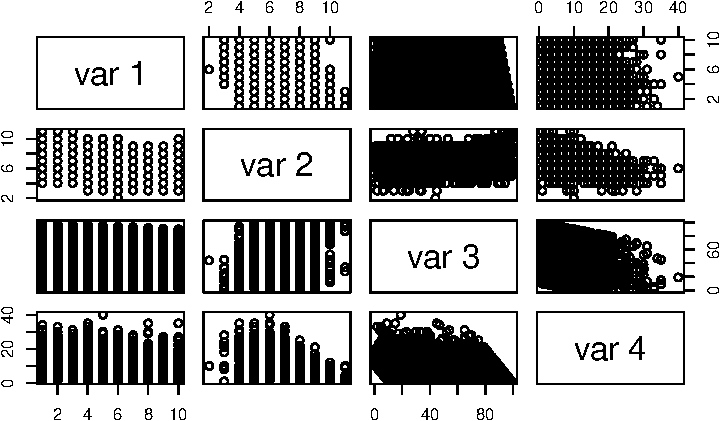
\includegraphics{project_report_files/figure-pdf/unnamed-chunk-5-1.pdf}

}

\end{figure}

Upon evaluating our Decision Tree model, we observed its simplicity - it
comprises only one split. While simplicity can be a virtue, in this
case, it indicates that our model may be overly simplistic to capture
the complexities inherent in our dataset. This simplicity could stem
from the nuanced nature of the `Yards' variable in the dataset, which
might require a more sophisticated approach to uncover the underlying
patterns effectively.

Given this situation, we turn our attention to the Random Forest model.
A Random Forest is essentially an ensemble of Decision Trees. This
ensemble approach amalgamates the predictions from multiple trees,
thereby enhancing the model's ability to capture complex relationships
and reducing the risk of overfitting, which is a common challenge with
individual Decision Trees. By leveraging the collective wisdom of
multiple trees, a Random Forest can often achieve higher accuracy and
better generalization to new, unseen data.

We proceed to build and evaluate a Random Forest model on our dataset,
hoping to achieve better predictive performance than our initial
simplistic Decision Tree.

\begin{Shaded}
\begin{Highlighting}[]
\CommentTok{\# Building the Random Forest model}
\NormalTok{rf\_model }\OtherTok{\textless{}{-}} \FunctionTok{randomForest}\NormalTok{(Yards }\SpecialCharTok{\textasciitilde{}}\NormalTok{ ., }\AttributeTok{data =}\NormalTok{ train.set, }\AttributeTok{ntree =} \FloatTok{300.}\NormalTok{, }\AttributeTok{mtry =} \DecValTok{3}\NormalTok{)}

\CommentTok{\# Predicting on the test set}
\NormalTok{rf\_predictions }\OtherTok{\textless{}{-}} \FunctionTok{predict}\NormalTok{(rf\_model, test.set)}

\CommentTok{\# Evaluating the model using Root Mean Squared Error}
\NormalTok{rf\_rmse }\OtherTok{\textless{}{-}} \FunctionTok{sqrt}\NormalTok{(}\FunctionTok{mean}\NormalTok{((test.set}\SpecialCharTok{$}\NormalTok{Yards }\SpecialCharTok{{-}}\NormalTok{ rf\_predictions)}\SpecialCharTok{\^{}}\DecValTok{2}\NormalTok{))}

\CommentTok{\# Output the Root Mean Squared Error}
\NormalTok{rf\_rmse}
\end{Highlighting}
\end{Shaded}

\begin{verbatim}
[1] 7.803932
\end{verbatim}

\begin{Shaded}
\begin{Highlighting}[]
\CommentTok{\# Getting the importance of each variable based on IncNodePurity}
\NormalTok{feature\_importance }\OtherTok{\textless{}{-}} \FunctionTok{importance}\NormalTok{(rf\_model)}

\CommentTok{\# Sorting features by IncNodePurity and selecting the top 3}
\NormalTok{top\_features }\OtherTok{\textless{}{-}} \FunctionTok{sort}\NormalTok{(feature\_importance[, }\StringTok{\textquotesingle{}IncNodePurity\textquotesingle{}}\NormalTok{], }\AttributeTok{decreasing =} \ConstantTok{TRUE}\NormalTok{)[}\DecValTok{1}\SpecialCharTok{:}\DecValTok{3}\NormalTok{]}

\CommentTok{\# Output the top 3 important features}
\NormalTok{top\_features}
\end{Highlighting}
\end{Shaded}

\begin{verbatim}
YardsFromOwnGoal       ScoreDelta         Humidity 
        45757.40         36243.66         31581.34 
\end{verbatim}

Our models top 3 import predictors are \texttt{YardsFromOwnGoal},
\texttt{Temperature} and \texttt{Humidity}. Before commenting on these
results, we will build an XGBoost model to see if we can improve our
RMSE.

Next, we turn our focus to preparing the data for XGBoost, a powerful
gradient boosting framework. XGBoost requires the data to be in a matrix
format. Thus, we convert our training and testing datasets accordingly,
excluding the target variable `Yards'. This conversion is a critical
step in harnessing the full potential of XGBoost's capabilities.

\begin{Shaded}
\begin{Highlighting}[]
\CommentTok{\# Prepare the data for XGBoost}
\CommentTok{\# Convert data to matrix format as xgboost works with the matrix}
\NormalTok{train\_matrix }\OtherTok{\textless{}{-}} \FunctionTok{as.matrix}\NormalTok{(train.set[, }\SpecialCharTok{{-}}\FunctionTok{which}\NormalTok{(}\FunctionTok{names}\NormalTok{(train.set) }\SpecialCharTok{==} \StringTok{"Yards"}\NormalTok{)])}
\NormalTok{test\_matrix }\OtherTok{\textless{}{-}} \FunctionTok{as.matrix}\NormalTok{(test.set[, }\SpecialCharTok{{-}}\FunctionTok{which}\NormalTok{(}\FunctionTok{names}\NormalTok{(test.set) }\SpecialCharTok{==} \StringTok{"Yards"}\NormalTok{)])}

\CommentTok{\# Create DMatrices}
\NormalTok{dtrain }\OtherTok{\textless{}{-}} \FunctionTok{xgb.DMatrix}\NormalTok{(}\AttributeTok{data =}\NormalTok{ train\_matrix, }\AttributeTok{label =}\NormalTok{ train.set}\SpecialCharTok{$}\NormalTok{Yards)}
\NormalTok{dtest }\OtherTok{\textless{}{-}} \FunctionTok{xgb.DMatrix}\NormalTok{(}\AttributeTok{data =}\NormalTok{ test\_matrix, }\AttributeTok{label =}\NormalTok{ test.set}\SpecialCharTok{$}\NormalTok{Yards)}
\end{Highlighting}
\end{Shaded}

Now we can run the model:

\begin{Shaded}
\begin{Highlighting}[]
\CommentTok{\# Set XGBoost parameters}
\NormalTok{params }\OtherTok{\textless{}{-}} \FunctionTok{list}\NormalTok{(}
    \AttributeTok{booster =} \StringTok{"gbtree"}\NormalTok{,}
    \AttributeTok{objective =} \StringTok{"reg:squarederror"}\NormalTok{,  }\CommentTok{\# Objective function for regression}
    \AttributeTok{eta =} \FloatTok{0.1}\NormalTok{,                      }\CommentTok{\# Learning rate}
    \AttributeTok{max\_depth =} \DecValTok{6}\NormalTok{,                  }\CommentTok{\# Depth of trees}
    \AttributeTok{subsample =} \FloatTok{0.5}\NormalTok{,                }\CommentTok{\# Subsampling of the training data}
    \AttributeTok{colsample\_bytree =} \FloatTok{0.5}          \CommentTok{\# Subsampling of features}
\NormalTok{)}

\CommentTok{\# Number of boosting rounds}
\NormalTok{nrounds }\OtherTok{\textless{}{-}} \DecValTok{100}

\CommentTok{\# Train the model}
\NormalTok{xgb\_model }\OtherTok{\textless{}{-}} \FunctionTok{xgb.train}\NormalTok{(}\AttributeTok{params =}\NormalTok{ params, }\AttributeTok{data =}\NormalTok{ dtrain, }\AttributeTok{nrounds =}\NormalTok{ nrounds)}

\CommentTok{\# Predicting}
\NormalTok{xgb\_predictions }\OtherTok{\textless{}{-}} \FunctionTok{predict}\NormalTok{(xgb\_model, dtest)}

\CommentTok{\# Evaluate the model}
\CommentTok{\# For example, using Root Mean Squared Error (RMSE)}
\NormalTok{true\_values }\OtherTok{\textless{}{-}}\NormalTok{ test.set}\SpecialCharTok{$}\NormalTok{Yards}
\NormalTok{rmse }\OtherTok{\textless{}{-}} \FunctionTok{sqrt}\NormalTok{(}\FunctionTok{mean}\NormalTok{((true\_values }\SpecialCharTok{{-}}\NormalTok{ xgb\_predictions)}\SpecialCharTok{\^{}}\DecValTok{2}\NormalTok{))}
\FunctionTok{print}\NormalTok{(}\FunctionTok{paste}\NormalTok{(}\StringTok{"RMSE:"}\NormalTok{, rmse))}
\end{Highlighting}
\end{Shaded}

\begin{verbatim}
[1] "RMSE: 7.82277337951654"
\end{verbatim}

Next we can plot a scatter plot of the actual vs predicted values:

\begin{Shaded}
\begin{Highlighting}[]
\CommentTok{\# Scatter plot of actual vs. predicted values}
\FunctionTok{plot}\NormalTok{(true\_values, xgb\_predictions, }\AttributeTok{main =} \StringTok{"Actual vs Predicted Yards"}\NormalTok{, }\AttributeTok{xlab =} \StringTok{"Actual Yards"}\NormalTok{, }\AttributeTok{ylab =} \StringTok{"Predicted Yards"}\NormalTok{, }\AttributeTok{pch =} \DecValTok{19}\NormalTok{)}
\FunctionTok{abline}\NormalTok{(}\DecValTok{0}\NormalTok{, }\DecValTok{1}\NormalTok{, }\AttributeTok{col =} \StringTok{"red"}\NormalTok{)  }\CommentTok{\# Adds a 45{-}degree line}
\end{Highlighting}
\end{Shaded}

\begin{figure}[H]

{\centering 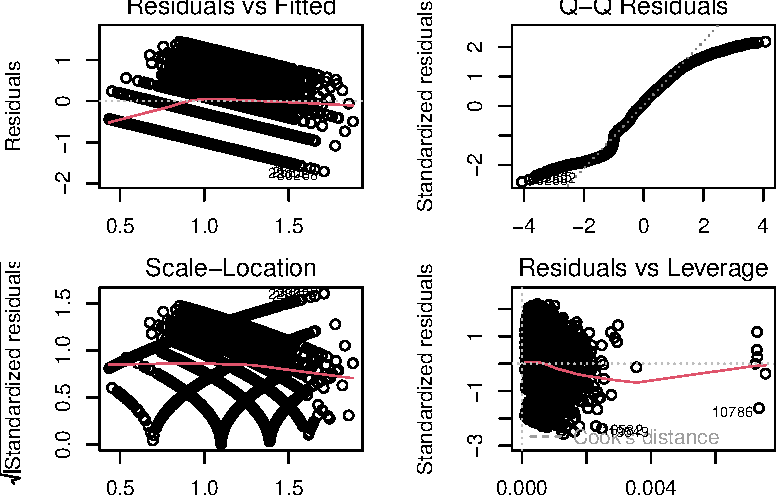
\includegraphics{project_report_files/figure-pdf/unnamed-chunk-9-1.pdf}

}

\end{figure}

As we can see, there are many outliers from plays where the running
backs break out and gain a lot of yards and also some outliers from
where thee running backs lose more than 5 yards. Similar to the approach
used in the previous modeling techniques, we will remove all plays where
the running back gained more than 10 yards and lost more than 5. This
will help us get a better understanding of the model's performance on
the majority of plays. The intuition behind this is two fold. Domain
knowledge helps us claim that not many plays end in either breakout or
major loss plays, but we can also look at the summary statistics of the
dataset to confirm this.

\begin{Shaded}
\begin{Highlighting}[]
\FunctionTok{summary}\NormalTok{(football\_data}\SpecialCharTok{$}\NormalTok{Yards)}
\end{Highlighting}
\end{Shaded}

\begin{verbatim}
   Min. 1st Qu.  Median    Mean 3rd Qu.    Max. 
-15.000   1.000   3.000   4.228   6.000  99.000 
\end{verbatim}

When we check these statistics we can see that 75\% of the data results
in a gain of 6 yards or less and 75\% of the data results in a gain of 1
yard or more. This confirms our intuition, and helps justify the
tresholds we set for the outliers.

Since we are only focused on the most common plays and not breakout
runs, we will remove any data of 10 yards or more. This is due to the
fact that plays resulting in 10 yards are considered to be just as
successful are play resulting in more than 10 yards. In addition, any
plays resulting in 0 or negative yards will be removed. This is due to
the fact that these plays are considered to be unsuccessful.

\begin{Shaded}
\begin{Highlighting}[]
\CommentTok{\# Remove any rows whose yards column is greater than 30}
\NormalTok{football\_data }\OtherTok{\textless{}{-}}\NormalTok{ football\_data[football\_data}\SpecialCharTok{$}\NormalTok{Yards }\SpecialCharTok{\textless{}=} \DecValTok{10} \SpecialCharTok{\&}\NormalTok{ football\_data}\SpecialCharTok{$}\NormalTok{Yards }\SpecialCharTok{\textgreater{}} \DecValTok{0}\NormalTok{, ]}
\end{Highlighting}
\end{Shaded}

We do not show the code as the model is the exact same, instead we only
show the output:

\begin{verbatim}
[1] "RMSE: 2.35698973331391"
\end{verbatim}

Again we can plot the actual vs predicted values:

\begin{Shaded}
\begin{Highlighting}[]
\CommentTok{\# Scatter plot of actual vs. predicted values}
\FunctionTok{plot}\NormalTok{(true\_values, xgb\_predictions, }\AttributeTok{main =} \StringTok{"Actual vs Predicted Yards"}\NormalTok{, }\AttributeTok{xlab =} \StringTok{"Actual Yards"}\NormalTok{, }\AttributeTok{ylab =} \StringTok{"Predicted Yards"}\NormalTok{, }\AttributeTok{pch =} \DecValTok{19}\NormalTok{)}
\FunctionTok{abline}\NormalTok{(}\DecValTok{0}\NormalTok{, }\DecValTok{1}\NormalTok{, }\AttributeTok{col =} \StringTok{"red"}\NormalTok{)  }\CommentTok{\# Adds a 45{-}degree line}
\end{Highlighting}
\end{Shaded}

\begin{figure}[H]

{\centering \includegraphics{project_report_files/figure-pdf/unnamed-chunk-13-1.pdf}

}

\end{figure}

We can also check feature importance, mean absolute error and the
residuals plot:

\begin{Shaded}
\begin{Highlighting}[]
\CommentTok{\# Variable importance plot}
\NormalTok{importance\_matrix }\OtherTok{\textless{}{-}} \FunctionTok{xgb.importance}\NormalTok{(}\AttributeTok{feature\_names =} \FunctionTok{colnames}\NormalTok{(train\_matrix), }\AttributeTok{model =}\NormalTok{ xgb\_model)}
\FunctionTok{xgb.plot.importance}\NormalTok{(importance\_matrix)}
\end{Highlighting}
\end{Shaded}

\begin{figure}[H]

{\centering \includegraphics{project_report_files/figure-pdf/unnamed-chunk-14-1.pdf}

}

\end{figure}

\begin{Shaded}
\begin{Highlighting}[]
\CommentTok{\# Mean Absolute Error}
\NormalTok{mae }\OtherTok{\textless{}{-}} \FunctionTok{mean}\NormalTok{(}\FunctionTok{abs}\NormalTok{(true\_values }\SpecialCharTok{{-}}\NormalTok{ xgb\_predictions))}
\FunctionTok{print}\NormalTok{(}\FunctionTok{paste}\NormalTok{(}\StringTok{"MAE:"}\NormalTok{, mae))}
\end{Highlighting}
\end{Shaded}

\begin{verbatim}
[1] "MAE: 1.90598015938816"
\end{verbatim}

\begin{Shaded}
\begin{Highlighting}[]
\CommentTok{\# Residuals plot}
\NormalTok{residuals }\OtherTok{\textless{}{-}}\NormalTok{ true\_values }\SpecialCharTok{{-}}\NormalTok{ xgb\_predictions}
\FunctionTok{plot}\NormalTok{(residuals, }\AttributeTok{type =} \StringTok{"l"}\NormalTok{, }\AttributeTok{main =} \StringTok{"Residuals Plot"}\NormalTok{, }\AttributeTok{xlab =} \StringTok{"Index"}\NormalTok{, }\AttributeTok{ylab =} \StringTok{"Residual"}\NormalTok{)}
\FunctionTok{abline}\NormalTok{(}\AttributeTok{h =} \DecValTok{0}\NormalTok{, }\AttributeTok{col =} \StringTok{"red"}\NormalTok{)}
\end{Highlighting}
\end{Shaded}

\begin{figure}[H]

{\centering \includegraphics{project_report_files/figure-pdf/unnamed-chunk-16-1.pdf}

}

\end{figure}

\hypertarget{analysis-of-results}{%
\subsubsection{Analysis of Results:}\label{analysis-of-results}}

\hypertarget{appendix}{%
\section{Appendix}\label{appendix}}

\hypertarget{multiple-linear-regression}{%
\subsection{Multiple Linear
Regression}\label{multiple-linear-regression}}

First, lets start by importing the completely clean and ready to use
dataset. This dataset was the result of procedures outlined in the data
cleaning and preprocessing section.

\begin{Shaded}
\begin{Highlighting}[]
\CommentTok{\# Import the dataset}
\NormalTok{football\_data }\OtherTok{\textless{}{-}} \FunctionTok{read.csv}\NormalTok{(}\StringTok{"/Users/giovanni{-}lunetta/uconn\_masters/stat5405/final\_project/data/train\_ready.csv"}\NormalTok{)}

\FunctionTok{str}\NormalTok{(football\_data)}
\end{Highlighting}
\end{Shaded}

\begin{verbatim}
'data.frame':   31007 obs. of  21 variables:
 $ Quarter          : int  2 2 4 2 2 1 2 4 4 4 ...
 $ Down             : int  1 1 1 2 1 1 1 1 1 1 ...
 $ Distance         : int  10 10 10 10 10 10 10 10 10 10 ...
 $ OffenseFormation : chr  "SINGLEBACK" "I_FORM" "I_FORM" "SINGLEBACK" ...
 $ RB               : int  2 2 2 1 1 1 1 1 2 1 ...
 $ TE               : int  1 1 2 1 1 2 1 1 1 1 ...
 $ WR               : int  2 2 1 3 3 2 3 3 1 3 ...
 $ DefendersInTheBox: int  8 7 8 6 7 8 6 7 7 7 ...
 $ Yards            : int  1 12 3 -2 14 4 3 7 7 3 ...
 $ Week             : int  3 9 14 2 2 2 17 11 17 3 ...
 $ GameWeather      : chr  "clear" "overcast" "clear" "clear" ...
 $ Temperature      : int  84 77 39 81 79 79 19 68 71 68 ...
 $ Humidity         : int  25 62 55 45 48 48 36 54 66 42 ...
 $ WindSpeed        : num  5 16 11 5 5 5 12 4 9 13 ...
 $ WindDirection    : chr  "west" "south east" "none" "east" ...
 $ GameHour         : int  15 9 3 3 13 12 2 6 15 12 ...
 $ DL               : int  4 3 4 4 2 4 2 4 4 4 ...
 $ LB               : int  3 4 3 2 4 3 4 2 3 2 ...
 $ BL               : int  4 4 4 5 5 4 5 5 4 5 ...
 $ YardsFromOwnGoal : int  40 84 79 21 86 25 49 25 65 54 ...
 $ ScoreDelta       : int  -7 0 -13 -11 0 7 -11 41 -16 -8 ...
\end{verbatim}

Since we are only focused on the most common plays and not breakout
runs, we will remove any data of 10 yards or more. This is due to the
fact that plays resulting in 10 yards are considered to be just as
successful are play resulting in more than 10 yards. In addition, any
plays resulting in 0 or negative yards will be removed. This is due to
the fact that these plays are considered to be unsuccessful.

\begin{Shaded}
\begin{Highlighting}[]
\CommentTok{\# Remove any rows whose yards column is greater than 30}
\NormalTok{football\_data }\OtherTok{\textless{}{-}}\NormalTok{ football\_data[football\_data}\SpecialCharTok{$}\NormalTok{Yards }\SpecialCharTok{\textless{}=} \DecValTok{10} \SpecialCharTok{\&}\NormalTok{ football\_data}\SpecialCharTok{$}\NormalTok{Yards }\SpecialCharTok{\textgreater{}} \DecValTok{0}\NormalTok{, ]}
\end{Highlighting}
\end{Shaded}

Lets now look at the histogram of Yards to get a better understanding of
the distribution of the response variable.

\begin{Shaded}
\begin{Highlighting}[]
\CommentTok{\# Histogram of Yards}
\FunctionTok{hist}\NormalTok{(football\_data}\SpecialCharTok{$}\NormalTok{Yards, }\AttributeTok{main =} \StringTok{"Histogram of Yards"}\NormalTok{, }\AttributeTok{xlab =} \StringTok{"Yards"}\NormalTok{, }\AttributeTok{ylab =} \StringTok{"Frequency"}\NormalTok{, }\AttributeTok{col =} \StringTok{"blue"}\NormalTok{)}
\end{Highlighting}
\end{Shaded}

\begin{figure}[H]

{\centering 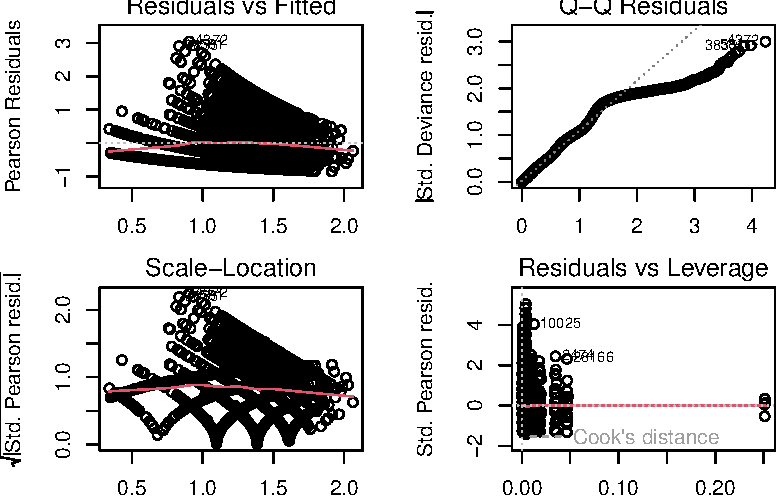
\includegraphics{project_report_files/figure-pdf/unnamed-chunk-19-1.pdf}

}

\end{figure}

Based on the histogram above, it is apparent that the number of yards is
skewed to the right. In order to address this issue, the Box-Cox
transformation will be utilized. This will help to normalize the
distribution of the response variable. The Box-Cox transformation can
transform non-normal data into normal data.

\begin{Shaded}
\begin{Highlighting}[]
\FunctionTok{library}\NormalTok{(MASS)}
\NormalTok{lambda\_null }\OtherTok{\textless{}{-}} \FunctionTok{boxcox}\NormalTok{(}\FunctionTok{lm}\NormalTok{(Yards }\SpecialCharTok{\textasciitilde{}} \DecValTok{1}\NormalTok{, }\AttributeTok{data =}\NormalTok{ football\_data))}
\end{Highlighting}
\end{Shaded}

\begin{figure}[H]

{\centering 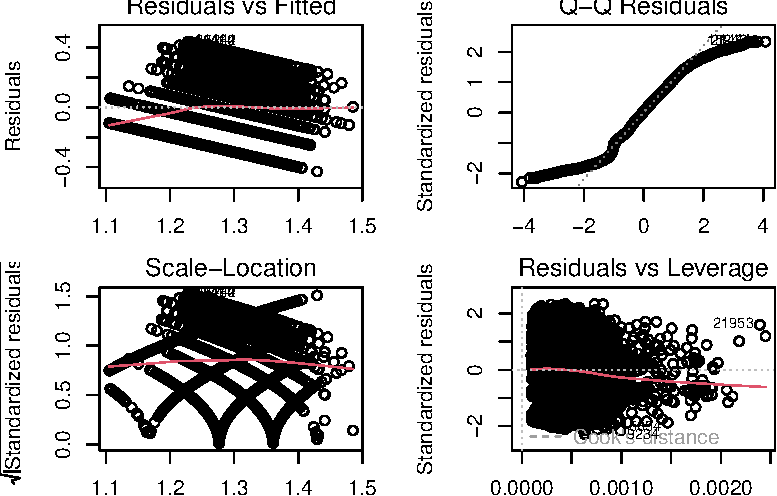
\includegraphics{project_report_files/figure-pdf/unnamed-chunk-20-1.pdf}

}

\end{figure}

The best lambda value for the Box-Cox tranformation is as follows:

\begin{Shaded}
\begin{Highlighting}[]
\NormalTok{lambda\_null}\SpecialCharTok{$}\NormalTok{x[}\FunctionTok{which.max}\NormalTok{(lambda\_null}\SpecialCharTok{$}\NormalTok{y)]}
\end{Highlighting}
\end{Shaded}

\begin{verbatim}
[1] 0.2222222
\end{verbatim}

Now the Box-Cox tranformation will be applied to the variable Yards with
the best lambda value.

\begin{Shaded}
\begin{Highlighting}[]
\NormalTok{lm\_model\_null }\OtherTok{\textless{}{-}} \FunctionTok{lm}\NormalTok{((Yards}\SpecialCharTok{\^{}}\NormalTok{(lambda\_null}\SpecialCharTok{$}\NormalTok{x[}\FunctionTok{which.max}\NormalTok{(lambda\_null}\SpecialCharTok{$}\NormalTok{y)])) }\SpecialCharTok{\textasciitilde{}} \DecValTok{1}\NormalTok{, }\AttributeTok{data =}\NormalTok{ football\_data)}
\FunctionTok{summary}\NormalTok{(lm\_model\_null)}
\end{Highlighting}
\end{Shaded}

\begin{verbatim}

Call:
lm(formula = (Yards^(lambda_null$x[which.max(lambda_null$y)])) ~ 
    1, data = football_data)

Residuals:
     Min       1Q   Median       3Q      Max 
-0.30438 -0.13785 -0.02786  0.12559  0.36373 

Coefficients:
            Estimate Std. Error t value Pr(>|t|)    
(Intercept)   1.3044     0.0013    1003   <2e-16 ***
---
Signif. codes:  0 '***' 0.001 '**' 0.01 '*' 0.05 '.' 0.1 ' ' 1

Residual standard error: 0.1924 on 21900 degrees of freedom
\end{verbatim}

Now the full model using all of the predictors will be created. In this
full model, there will be 0 interactions between the predictors. The
same process using the Box-Cox transformation will be used to normalize
the distribution of the response variable.

\begin{Shaded}
\begin{Highlighting}[]
\NormalTok{lambda\_full }\OtherTok{\textless{}{-}} \FunctionTok{boxcox}\NormalTok{(}\FunctionTok{lm}\NormalTok{(Yards }\SpecialCharTok{\textasciitilde{}}\NormalTok{ ., }\AttributeTok{data =}\NormalTok{ football\_data))}
\end{Highlighting}
\end{Shaded}

\begin{figure}[H]

{\centering \includegraphics{project_report_files/figure-pdf/unnamed-chunk-23-1.pdf}

}

\end{figure}

The best lambda value for the Box-Cox tranformation is as follows:

\begin{Shaded}
\begin{Highlighting}[]
\NormalTok{lambda\_full}\SpecialCharTok{$}\NormalTok{x[}\FunctionTok{which.max}\NormalTok{(lambda\_full}\SpecialCharTok{$}\NormalTok{y)]}
\end{Highlighting}
\end{Shaded}

\begin{verbatim}
[1] 0.2222222
\end{verbatim}

Now the Box-Cox tranformation will be applied to the variable Yards with
the best lambda value.

\begin{Shaded}
\begin{Highlighting}[]
\NormalTok{lm\_model\_full }\OtherTok{\textless{}{-}} \FunctionTok{lm}\NormalTok{((Yards}\SpecialCharTok{\^{}}\NormalTok{(lambda\_full}\SpecialCharTok{$}\NormalTok{x[}\FunctionTok{which.max}\NormalTok{(lambda\_full}\SpecialCharTok{$}\NormalTok{y)])) }\SpecialCharTok{\textasciitilde{}}\NormalTok{ ., }\AttributeTok{data =}\NormalTok{ football\_data)}
\FunctionTok{summary}\NormalTok{(lm\_model\_full)}
\end{Highlighting}
\end{Shaded}

\begin{verbatim}

Call:
lm(formula = (Yards^(lambda_full$x[which.max(lambda_full$y)])) ~ 
    ., data = football_data)

Residuals:
    Min      1Q  Median      3Q     Max 
-0.4747 -0.1367  0.0041  0.1391  0.5492 

Coefficients:
                             Estimate Std. Error t value Pr(>|t|)    
(Intercept)                 1.533e+00  4.252e-01   3.605 0.000313 ***
Quarter                     2.045e-04  1.118e-03   0.183 0.854945    
Down                        5.107e-03  2.244e-03   2.276 0.022858 *  
Distance                    3.834e-03  4.131e-04   9.281  < 2e-16 ***
OffenseFormationEMPTY       2.448e-02  1.924e-01   0.127 0.898746    
OffenseFormationI_FORM     -1.747e-02  1.882e-01  -0.093 0.926043    
OffenseFormationJUMBO      -1.027e-01  1.885e-01  -0.545 0.585728    
OffenseFormationPISTOL     -1.521e-02  1.883e-01  -0.081 0.935626    
OffenseFormationSHOTGUN    -2.954e-02  1.882e-01  -0.157 0.875255    
OffenseFormationSINGLEBACK -1.847e-02  1.882e-01  -0.098 0.921801    
OffenseFormationUNKNOWN    -4.269e-02  2.104e-01  -0.203 0.839222    
OffenseFormationWILDCAT    -1.580e-04  1.898e-01  -0.001 0.999336    
RB                         -3.485e-03  5.875e-03  -0.593 0.553054    
TE                         -1.421e-03  4.898e-03  -0.290 0.771792    
WR                         -6.871e-03  4.992e-03  -1.377 0.168679    
DefendersInTheBox          -2.749e-02  1.945e-03 -14.135  < 2e-16 ***
Week                       -2.282e-04  3.435e-04  -0.664 0.506415    
GameWeathernone             7.253e-03  4.231e-03   1.714 0.086506 .  
GameWeatherovercast        -3.271e-04  3.110e-03  -0.105 0.916235    
GameWeatherrain            -4.791e-03  6.303e-03  -0.760 0.447222    
GameWeathersnow            -8.656e-03  1.815e-02  -0.477 0.633395    
Temperature                -3.019e-04  1.007e-04  -2.997 0.002725 ** 
Humidity                   -2.216e-05  6.295e-05  -0.352 0.724800    
WindSpeed                   1.854e-05  3.094e-04   0.060 0.952216    
WindDirectionnone          -9.389e-03  8.146e-03  -1.153 0.249086    
WindDirectionnorth         -2.802e-03  9.503e-03  -0.295 0.768153    
WindDirectionnorth east    -8.067e-03  8.197e-03  -0.984 0.325065    
WindDirectionnorth west    -4.240e-03  8.276e-03  -0.512 0.608408    
WindDirectionsouth         -7.687e-03  9.009e-03  -0.853 0.393538    
WindDirectionsouth east    -4.907e-03  8.529e-03  -0.575 0.565104    
WindDirectionsouth west    -5.235e-03  8.041e-03  -0.651 0.515082    
WindDirectionwest          -5.371e-03  9.581e-03  -0.561 0.575079    
GameHour                    5.345e-04  2.913e-04   1.835 0.066531 .  
DL                         -2.015e-03  3.461e-02  -0.058 0.953559    
LB                         -3.061e-03  3.469e-02  -0.088 0.929677    
BL                          5.420e-03  3.469e-02   0.156 0.875840    
YardsFromOwnGoal           -4.017e-04  5.336e-05  -7.529 5.33e-14 ***
ScoreDelta                 -2.177e-04  1.202e-04  -1.812 0.070023 .  
---
Signif. codes:  0 '***' 0.001 '**' 0.01 '*' 0.05 '.' 0.1 ' ' 1

Residual standard error: 0.1881 on 21863 degrees of freedom
Multiple R-squared:  0.04641,   Adjusted R-squared:  0.04479 
F-statistic: 28.76 on 37 and 21863 DF,  p-value: < 2.2e-16
\end{verbatim}

Based on the results of the full model, the model shows which predictors
are statistically significant. The most significant predictors are
Distance, DefendersInTheBox, and YardsFromOwnGoal. Creating scatter
plots of the response variable versus each of these predictors will help
to gain a better understanding of how these variables affect the
predicted yards.

\begin{Shaded}
\begin{Highlighting}[]
\CommentTok{\# Scatter plot of yards vs. Distance}
\FunctionTok{plot}\NormalTok{(football\_data}\SpecialCharTok{$}\NormalTok{Yards, football\_data}\SpecialCharTok{$}\NormalTok{Distance, }\AttributeTok{main =} \StringTok{"Yards vs. Distance"}\NormalTok{, }\AttributeTok{xlab =} \StringTok{"Yards"}\NormalTok{, }\AttributeTok{ylab =} \StringTok{"Distance"}\NormalTok{, }\AttributeTok{pch =} \DecValTok{19}\NormalTok{)}
\end{Highlighting}
\end{Shaded}

\begin{figure}[H]

{\centering 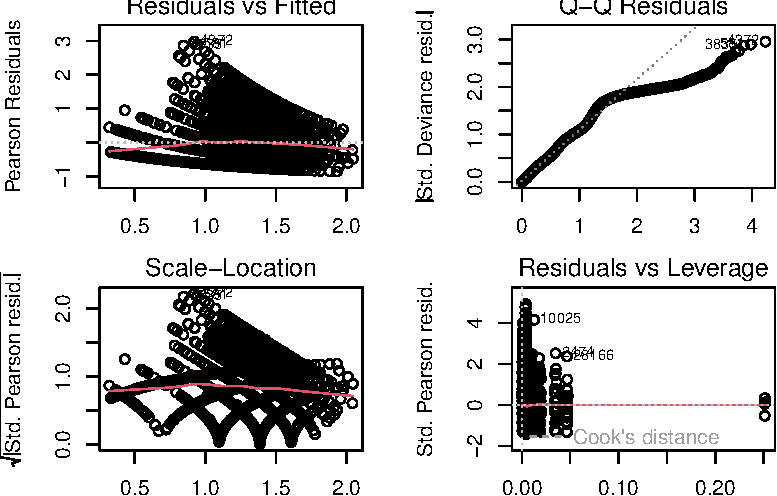
\includegraphics{project_report_files/figure-pdf/unnamed-chunk-26-1.pdf}

}

\end{figure}

Looking at this scatter plot of Yards vs Distance, there appears to only
be a sinusoial relationship between the two variables. Therefore, when a
reduced model is created, a sine function will be used to model the
relationship between the two variables.

\begin{Shaded}
\begin{Highlighting}[]
\CommentTok{\# Scatter plot of yards vs. Defenders In The Box}
\FunctionTok{plot}\NormalTok{(football\_data}\SpecialCharTok{$}\NormalTok{Yards, football\_data}\SpecialCharTok{$}\NormalTok{DefendersInTheBox, }\AttributeTok{main =} \StringTok{"Yards vs. Defenders In The Box"}\NormalTok{, }\AttributeTok{xlab =} \StringTok{"Yards"}\NormalTok{, }\AttributeTok{ylab =} \StringTok{"Defenders In The Box"}\NormalTok{, }\AttributeTok{pch =} \DecValTok{19}\NormalTok{)}
\end{Highlighting}
\end{Shaded}

\begin{figure}[H]

{\centering \includegraphics{project_report_files/figure-pdf/unnamed-chunk-27-1.pdf}

}

\end{figure}

Looking at this scatter plot of Yards vs Defenders In The Box, there
appears to be a quadratic function relationship between the two
variables. Therefore, when a reduced model is created, the Defenders In
The Box variable will be squared in order to capture this relationship

\begin{Shaded}
\begin{Highlighting}[]
\CommentTok{\# Scatter plot of yards vs. YardsFromOwnGoal}
\FunctionTok{plot}\NormalTok{(football\_data}\SpecialCharTok{$}\NormalTok{Yards, football\_data}\SpecialCharTok{$}\NormalTok{YardsFromOwnGoal, }\AttributeTok{main =} \StringTok{"Yards vs. Yards From Own Goal"}\NormalTok{, }\AttributeTok{xlab =} \StringTok{"Yards"}\NormalTok{, }\AttributeTok{ylab =} \StringTok{"Yards From Own Goal"}\NormalTok{, }\AttributeTok{pch =} \DecValTok{19}\NormalTok{)}
\end{Highlighting}
\end{Shaded}

\begin{figure}[H]

{\centering \includegraphics{project_report_files/figure-pdf/unnamed-chunk-28-1.pdf}

}

\end{figure}

The scatterplot of Yards vs Yards From Own Goal shows that there is a
linear relationship between the two variables. Therefore, when a reduced
model is created, the Yards From Own Goal variable will not be changed
since the model is already capturing this linear relationship.

In order to capture these relationships between variables, a new, full
model will be synthesized. This model will include the Distance variable
with a sine function and the Defenders In The Box variable squared.
However, the Box-Cox transformation will need to be run again.

\begin{Shaded}
\begin{Highlighting}[]
\NormalTok{lambda\_full }\OtherTok{\textless{}{-}} \FunctionTok{boxcox}\NormalTok{(}\FunctionTok{lm}\NormalTok{(Yards }\SpecialCharTok{\textasciitilde{}}\NormalTok{ Quarter }\SpecialCharTok{+}\NormalTok{ Down }\SpecialCharTok{+} \FunctionTok{sin}\NormalTok{(Distance) }\SpecialCharTok{+}\NormalTok{ OffenseFormation }\SpecialCharTok{+}\NormalTok{ RB }\SpecialCharTok{+}\NormalTok{ TE }\SpecialCharTok{+}\NormalTok{ WR }\SpecialCharTok{+}\NormalTok{ DefendersInTheBox}\SpecialCharTok{\^{}}\DecValTok{2} \SpecialCharTok{+}\NormalTok{ Week }\SpecialCharTok{+}\NormalTok{ GameWeather }\SpecialCharTok{+}\NormalTok{ Temperature }\SpecialCharTok{+}\NormalTok{ Humidity }\SpecialCharTok{+}\NormalTok{ WindSpeed }\SpecialCharTok{+}\NormalTok{ WindDirection }\SpecialCharTok{+}\NormalTok{ GameHour }\SpecialCharTok{+}\NormalTok{ DL }\SpecialCharTok{+}\NormalTok{ LB }\SpecialCharTok{+}\NormalTok{ BL }\SpecialCharTok{+}\NormalTok{ YardsFromOwnGoal }\SpecialCharTok{+}\NormalTok{ ScoreDelta, }\AttributeTok{data =}\NormalTok{ football\_data))}
\end{Highlighting}
\end{Shaded}

\begin{figure}[H]

{\centering 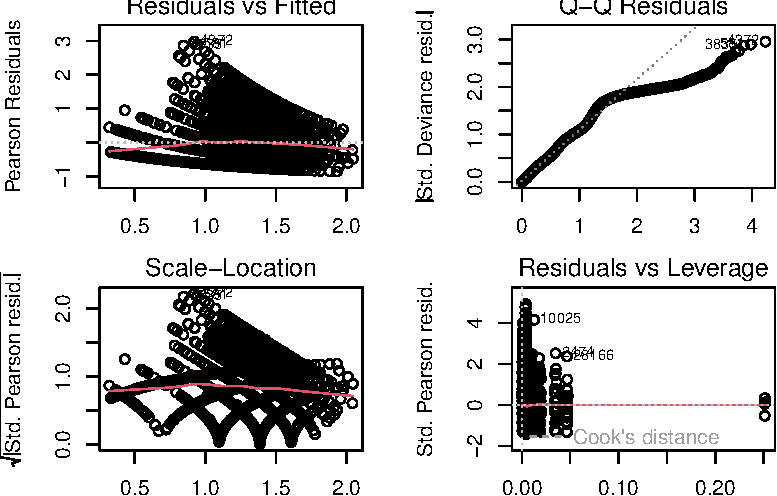
\includegraphics{project_report_files/figure-pdf/unnamed-chunk-29-1.pdf}

}

\end{figure}

\begin{Shaded}
\begin{Highlighting}[]
\FunctionTok{summary}\NormalTok{(lambda\_full)}
\end{Highlighting}
\end{Shaded}

\begin{verbatim}
  Length Class  Mode   
x 100    -none- numeric
y 100    -none- numeric
\end{verbatim}

The best lambda value for the Box-Cox tranformation is as follows:

\begin{Shaded}
\begin{Highlighting}[]
\NormalTok{lambda\_full}\SpecialCharTok{$}\NormalTok{x[}\FunctionTok{which.max}\NormalTok{(lambda\_full}\SpecialCharTok{$}\NormalTok{y)]}
\end{Highlighting}
\end{Shaded}

\begin{verbatim}
[1] 0.2222222
\end{verbatim}

Now the Box-Cox tranformation will be applied to the variable Yards with
the best lambda value.

\begin{Shaded}
\begin{Highlighting}[]
\NormalTok{lm\_model\_full }\OtherTok{\textless{}{-}} \FunctionTok{lm}\NormalTok{((Yards}\SpecialCharTok{\^{}}\NormalTok{(lambda\_full}\SpecialCharTok{$}\NormalTok{x[}\FunctionTok{which.max}\NormalTok{(lambda\_full}\SpecialCharTok{$}\NormalTok{y)])) }\SpecialCharTok{\textasciitilde{}}\NormalTok{ Quarter }\SpecialCharTok{+}\NormalTok{ Down }\SpecialCharTok{+} \FunctionTok{sin}\NormalTok{(Distance) }\SpecialCharTok{+}\NormalTok{ OffenseFormation }\SpecialCharTok{+}\NormalTok{ RB }\SpecialCharTok{+}\NormalTok{ TE }\SpecialCharTok{+}\NormalTok{ WR }\SpecialCharTok{+}\NormalTok{ DefendersInTheBox}\SpecialCharTok{\^{}}\DecValTok{2} \SpecialCharTok{+}\NormalTok{ Week }\SpecialCharTok{+}\NormalTok{ GameWeather }\SpecialCharTok{+}\NormalTok{ Temperature }\SpecialCharTok{+}\NormalTok{ Humidity }\SpecialCharTok{+}\NormalTok{ WindSpeed }\SpecialCharTok{+}\NormalTok{ WindDirection }\SpecialCharTok{+}\NormalTok{ GameHour }\SpecialCharTok{+}\NormalTok{ DL }\SpecialCharTok{+}\NormalTok{ LB }\SpecialCharTok{+}\NormalTok{ BL }\SpecialCharTok{+}\NormalTok{ YardsFromOwnGoal }\SpecialCharTok{+}\NormalTok{ ScoreDelta, }\AttributeTok{data =}\NormalTok{ football\_data)}
\FunctionTok{summary}\NormalTok{(lm\_model\_full)}
\end{Highlighting}
\end{Shaded}

\begin{verbatim}

Call:
lm(formula = (Yards^(lambda_full$x[which.max(lambda_full$y)])) ~ 
    Quarter + Down + sin(Distance) + OffenseFormation + RB + 
        TE + WR + DefendersInTheBox^2 + Week + GameWeather + 
        Temperature + Humidity + WindSpeed + WindDirection + 
        GameHour + DL + LB + BL + YardsFromOwnGoal + ScoreDelta, 
    data = football_data)

Residuals:
     Min       1Q   Median       3Q      Max 
-0.43047 -0.13761  0.00579  0.13964  0.54723 

Coefficients:
                             Estimate Std. Error t value Pr(>|t|)    
(Intercept)                 1.572e+00  4.257e-01   3.693 0.000222 ***
Quarter                     4.560e-04  1.119e-03   0.407 0.683760    
Down                        6.823e-04  2.260e-03   0.302 0.762764    
sin(Distance)              -1.309e-02  2.557e-03  -5.118 3.11e-07 ***
OffenseFormationEMPTY       1.810e-02  1.926e-01   0.094 0.925163    
OffenseFormationI_FORM     -2.044e-02  1.885e-01  -0.108 0.913627    
OffenseFormationJUMBO      -1.057e-01  1.888e-01  -0.560 0.575549    
OffenseFormationPISTOL     -1.896e-02  1.886e-01  -0.101 0.919903    
OffenseFormationSHOTGUN    -3.184e-02  1.884e-01  -0.169 0.865822    
OffenseFormationSINGLEBACK -2.233e-02  1.884e-01  -0.119 0.905657    
OffenseFormationUNKNOWN    -4.517e-02  2.107e-01  -0.214 0.830241    
OffenseFormationWILDCAT    -3.616e-03  1.901e-01  -0.019 0.984823    
RB                         -3.657e-03  5.883e-03  -0.622 0.534153    
TE                         -9.796e-04  4.904e-03  -0.200 0.841678    
WR                         -7.130e-03  4.999e-03  -1.426 0.153781    
DefendersInTheBox          -2.953e-02  1.930e-03 -15.301  < 2e-16 ***
Week                       -1.953e-04  3.439e-04  -0.568 0.570043    
GameWeathernone             7.612e-03  4.237e-03   1.797 0.072415 .  
GameWeatherovercast        -2.761e-04  3.114e-03  -0.089 0.929343    
GameWeatherrain            -4.145e-03  6.312e-03  -0.657 0.511335    
GameWeathersnow            -7.028e-03  1.817e-02  -0.387 0.698943    
Temperature                -2.819e-04  1.008e-04  -2.795 0.005193 ** 
Humidity                   -3.439e-05  6.302e-05  -0.546 0.585250    
WindSpeed                   7.867e-05  3.097e-04   0.254 0.799487    
WindDirectionnone          -8.918e-03  8.157e-03  -1.093 0.274260    
WindDirectionnorth         -2.268e-03  9.516e-03  -0.238 0.811644    
WindDirectionnorth east    -7.485e-03  8.208e-03  -0.912 0.361843    
WindDirectionnorth west    -3.958e-03  8.287e-03  -0.478 0.632975    
WindDirectionsouth         -7.636e-03  9.021e-03  -0.846 0.397306    
WindDirectionsouth east    -4.302e-03  8.541e-03  -0.504 0.614508    
WindDirectionsouth west    -5.156e-03  8.052e-03  -0.640 0.521962    
WindDirectionwest          -4.050e-03  9.593e-03  -0.422 0.672902    
GameHour                    4.157e-04  2.914e-04   1.427 0.153660    
DL                         -1.108e-03  3.465e-02  -0.032 0.974487    
LB                         -1.580e-03  3.473e-02  -0.045 0.963712    
BL                          7.304e-03  3.473e-02   0.210 0.833457    
YardsFromOwnGoal           -4.871e-04  5.229e-05  -9.315  < 2e-16 ***
ScoreDelta                 -2.299e-04  1.203e-04  -1.911 0.055994 .  
---
Signif. codes:  0 '***' 0.001 '**' 0.01 '*' 0.05 '.' 0.1 ' ' 1

Residual standard error: 0.1883 on 21863 degrees of freedom
Multiple R-squared:  0.0438,    Adjusted R-squared:  0.04218 
F-statistic: 27.06 on 37 and 21863 DF,  p-value: < 2.2e-16
\end{verbatim}

Now lets use the step function to find the best model for the data.

\begin{Shaded}
\begin{Highlighting}[]
\NormalTok{lm\_model\_step }\OtherTok{\textless{}{-}} \FunctionTok{step}\NormalTok{(lm\_model\_full, }\AttributeTok{direction =} \StringTok{"backward"}\NormalTok{)}
\FunctionTok{summary}\NormalTok{(lm\_model\_step)}
\end{Highlighting}
\end{Shaded}

This new reduced model needs to be run similar to that of the previous
models utilizing the Box-Cox transformation.

\begin{Shaded}
\begin{Highlighting}[]
\NormalTok{lambda\_reduced }\OtherTok{\textless{}{-}} \FunctionTok{boxcox}\NormalTok{(}\FunctionTok{lm}\NormalTok{(Yards }\SpecialCharTok{\textasciitilde{}} \FunctionTok{sin}\NormalTok{(Distance) }\SpecialCharTok{+}\NormalTok{ WR }\SpecialCharTok{+}\NormalTok{ DefendersInTheBox}\SpecialCharTok{\^{}}\DecValTok{2} \SpecialCharTok{+}\NormalTok{ Temperature }\SpecialCharTok{+}\NormalTok{ BL }\SpecialCharTok{+}\NormalTok{ YardsFromOwnGoal, }\AttributeTok{data =}\NormalTok{ football\_data))}
\end{Highlighting}
\end{Shaded}

\begin{figure}[H]

{\centering \includegraphics{project_report_files/figure-pdf/unnamed-chunk-33-1.pdf}

}

\end{figure}

The best lambda value for the Box-Cox tranformation is as follows:

\begin{Shaded}
\begin{Highlighting}[]
\NormalTok{lambda\_reduced}\SpecialCharTok{$}\NormalTok{x[}\FunctionTok{which.max}\NormalTok{(lambda\_reduced}\SpecialCharTok{$}\NormalTok{y)]}
\end{Highlighting}
\end{Shaded}

\begin{verbatim}
[1] 0.2222222
\end{verbatim}

Now the Box-Cox tranformation will be applied to the variable Yards with
the best lambda value.

\begin{Shaded}
\begin{Highlighting}[]
\NormalTok{lm\_model\_reduced }\OtherTok{\textless{}{-}} \FunctionTok{lm}\NormalTok{((Yards}\SpecialCharTok{\^{}}\NormalTok{(lambda\_reduced}\SpecialCharTok{$}\NormalTok{x[}\FunctionTok{which.max}\NormalTok{(lambda\_reduced}\SpecialCharTok{$}\NormalTok{y)])) }\SpecialCharTok{\textasciitilde{}} \FunctionTok{sin}\NormalTok{(Distance) }\SpecialCharTok{+}\NormalTok{ WR }\SpecialCharTok{+}\NormalTok{ DefendersInTheBox}\SpecialCharTok{\^{}}\DecValTok{2} \SpecialCharTok{+}\NormalTok{ Temperature }\SpecialCharTok{+}\NormalTok{ BL }\SpecialCharTok{+}\NormalTok{ YardsFromOwnGoal, }\AttributeTok{data =}\NormalTok{ football\_data)}
\FunctionTok{summary}\NormalTok{(lm\_model\_reduced)}
\end{Highlighting}
\end{Shaded}

\begin{verbatim}

Call:
lm(formula = (Yards^(lambda_reduced$x[which.max(lambda_reduced$y)])) ~ 
    sin(Distance) + WR + DefendersInTheBox^2 + Temperature + 
        BL + YardsFromOwnGoal, data = football_data)

Residuals:
     Min       1Q   Median       3Q      Max 
-0.42892 -0.13844  0.00668  0.14027  0.47618 

Coefficients:
                    Estimate Std. Error t value Pr(>|t|)    
(Intercept)        1.518e+00  2.254e-02  67.351  < 2e-16 ***
sin(Distance)     -1.536e-02  2.198e-03  -6.989 2.85e-12 ***
WR                -5.522e-03  2.406e-03  -2.295 0.021750 *  
DefendersInTheBox -3.049e-02  1.865e-03 -16.345  < 2e-16 ***
Temperature       -2.167e-04  7.435e-05  -2.914 0.003574 ** 
BL                 9.724e-03  2.939e-03   3.309 0.000939 ***
YardsFromOwnGoal  -5.382e-04  5.167e-05 -10.417  < 2e-16 ***
---
Signif. codes:  0 '***' 0.001 '**' 0.01 '*' 0.05 '.' 0.1 ' ' 1

Residual standard error: 0.1886 on 21894 degrees of freedom
Multiple R-squared:  0.0394,    Adjusted R-squared:  0.03914 
F-statistic: 149.7 on 6 and 21894 DF,  p-value: < 2.2e-16
\end{verbatim}

By creating a Residuals vs Fitted plot, a Q-Q Residuals plot, a
Scale-Location plot, and a Residuals vs Leverage plot, the assumptions
of the model can be checked.

\begin{Shaded}
\begin{Highlighting}[]
\FunctionTok{par}\NormalTok{(}\AttributeTok{mfrow =} \FunctionTok{c}\NormalTok{(}\DecValTok{2}\NormalTok{, }\DecValTok{2}\NormalTok{))}
\NormalTok{old.par }\OtherTok{=} \FunctionTok{par}\NormalTok{(}\AttributeTok{mar =} \FunctionTok{c}\NormalTok{(}\DecValTok{3}\NormalTok{, }\DecValTok{4}\NormalTok{, }\DecValTok{1}\NormalTok{, }\DecValTok{2}\NormalTok{))}
\FunctionTok{plot}\NormalTok{(lm\_model\_reduced)}
\end{Highlighting}
\end{Shaded}

\begin{figure}[H]

{\centering 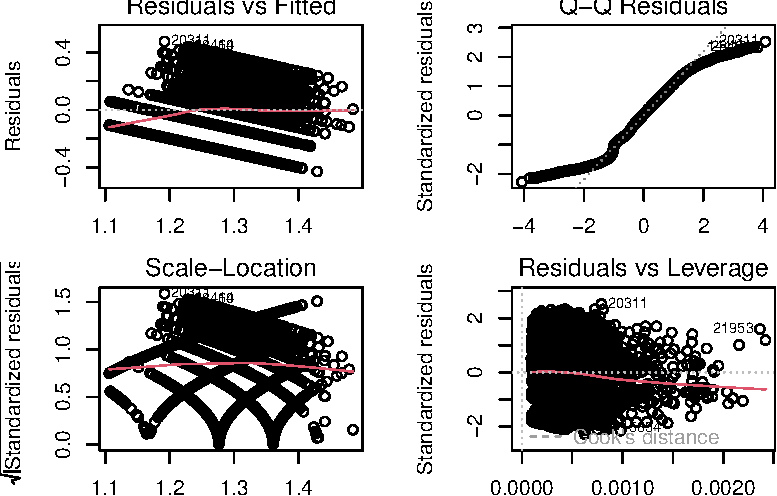
\includegraphics{project_report_files/figure-pdf/unnamed-chunk-36-1.pdf}

}

\end{figure}

Based on the plots above, the normality assumption is not violated, as
the Q-Q Residuals plot shows that the residuals are mainly normally
distributed.

In order to gain a better understanding of how these variables affect
the predicted yards, scatter plots of the predicted yards versus each of
the predictors will be created. However, the only scatter plots that
will be synthesized are those that have the three highest t values:
Distance, DefendersInTheBox, and YardsFromOwnGoal.

\begin{Shaded}
\begin{Highlighting}[]
\NormalTok{football\_data}\SpecialCharTok{$}\NormalTok{predicted\_yards }\OtherTok{\textless{}{-}} \FunctionTok{predict}\NormalTok{(lm\_model\_reduced, football\_data)}
\end{Highlighting}
\end{Shaded}

\begin{Shaded}
\begin{Highlighting}[]
\CommentTok{\# Scatter plot of predicted yards vs. Distance}
\FunctionTok{plot}\NormalTok{(football\_data}\SpecialCharTok{$}\NormalTok{predicted\_yards, football\_data}\SpecialCharTok{$}\NormalTok{Distance, }\AttributeTok{main =} \StringTok{"Predicted Yards vs. Distance"}\NormalTok{, }\AttributeTok{xlab =} \StringTok{"Predicted Yards"}\NormalTok{, }\AttributeTok{ylab =} \StringTok{"Distance"}\NormalTok{, }\AttributeTok{pch =} \DecValTok{19}\NormalTok{)}
\FunctionTok{abline}\NormalTok{(}\DecValTok{0}\NormalTok{, }\DecValTok{1}\NormalTok{, }\AttributeTok{col =} \StringTok{"red"}\NormalTok{)  }\CommentTok{\# Adds a 45{-}degree line}
\end{Highlighting}
\end{Shaded}

\begin{figure}[H]

{\centering 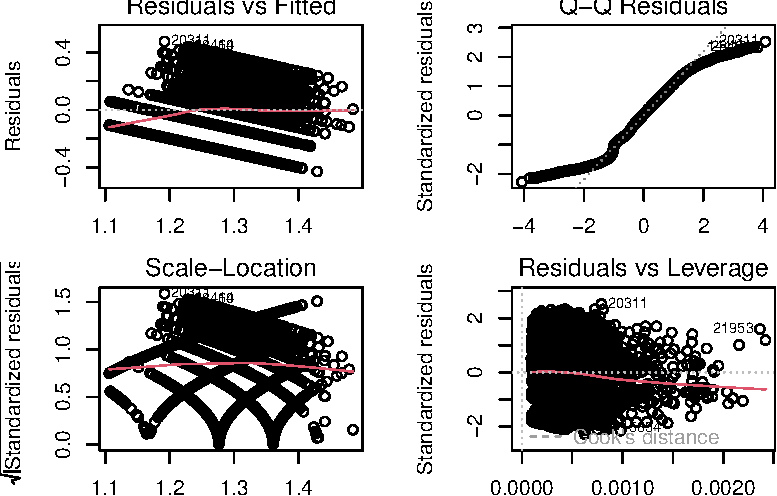
\includegraphics{project_report_files/figure-pdf/unnamed-chunk-38-1.pdf}

}

\end{figure}

\begin{Shaded}
\begin{Highlighting}[]
\CommentTok{\# Scatter plot of predicted yards vs. DefendersInTheBox}
\FunctionTok{plot}\NormalTok{(football\_data}\SpecialCharTok{$}\NormalTok{predicted\_yards, football\_data}\SpecialCharTok{$}\NormalTok{DefendersInTheBox, }\AttributeTok{main =} \StringTok{"Predicted Yards vs. DefendersInTheBox"}\NormalTok{, }\AttributeTok{xlab =} \StringTok{"Predicted Yards"}\NormalTok{, }\AttributeTok{ylab =} \StringTok{"DefendersInTheBox"}\NormalTok{, }\AttributeTok{pch =} \DecValTok{19}\NormalTok{)}
\FunctionTok{abline}\NormalTok{(}\DecValTok{0}\NormalTok{, }\DecValTok{1}\NormalTok{, }\AttributeTok{col =} \StringTok{"red"}\NormalTok{)  }\CommentTok{\# Adds a 45{-}degree line}
\end{Highlighting}
\end{Shaded}

\begin{figure}[H]

{\centering \includegraphics{project_report_files/figure-pdf/unnamed-chunk-39-1.pdf}

}

\end{figure}

\begin{Shaded}
\begin{Highlighting}[]
\CommentTok{\# Scatter plot of predicted yards vs. YardsFromOwnGoal}
\FunctionTok{plot}\NormalTok{(football\_data}\SpecialCharTok{$}\NormalTok{predicted\_yards, football\_data}\SpecialCharTok{$}\NormalTok{YardsFromOwnGoal, }\AttributeTok{main =} \StringTok{"Predicted Yards vs. YardsFromOwnGoal"}\NormalTok{, }\AttributeTok{xlab =} \StringTok{"Predicted Yards"}\NormalTok{, }\AttributeTok{ylab =} \StringTok{"YardsFromOwnGoal"}\NormalTok{, }\AttributeTok{pch =} \DecValTok{19}\NormalTok{)}
\FunctionTok{abline}\NormalTok{(}\DecValTok{0}\NormalTok{, }\DecValTok{1}\NormalTok{, }\AttributeTok{col =} \StringTok{"red"}\NormalTok{)  }\CommentTok{\# Adds a 45{-}degree line}
\end{Highlighting}
\end{Shaded}

\begin{figure}[H]

{\centering \includegraphics{project_report_files/figure-pdf/unnamed-chunk-40-1.pdf}

}

\end{figure}

\hypertarget{glm-with-gamma-response}{%
\subsection{GLM with Gamma Response}\label{glm-with-gamma-response}}

The next model that will be synthesized is a GLM with a gamma response.
The gamma distribution is a two-parameter family of continuous
probability distributions. The gamma distribution is a generalization of
the exponential distribution. The gamma distribution is frequently used
to model right-skewed data. The gamma distribution is a two-parameter
family of continuous probability distributions. The gamma distribution
is a generalization of the exponential distribution. The gamma
distribution is frequently used to model right-skewed data. The gamma
distribution is a two-parameter family of continuous probability
distributions. The gamma distribution is a generalization of the
exponential distribution. The gamma distribution is frequently used to
model right-skewed data. The gamma distribution is a two-parameter
family of continuous probability distributions. The gamma distribution
is a generalization of the exponential distribution. The gamma
distribution is frequently used to model right-skewed data. The gamma
distribution is a two-parameter family of continuous probability
distributions. The gamma distribution is a generalization of the
exponential distribution. The gamma distribution is frequently used to
model right-skewed data. The gamma distribution is a two-parameter
family of continuous probability distributions. The gamma distribution
is a generalization of the exponential distribution. The gamma
distribution is frequently used to model right-skewed data.

Lets start by removing any rows whose yards column is negative. This is
because the gamma distribution cannot have negative values.

\begin{Shaded}
\begin{Highlighting}[]
\CommentTok{\# Remove any rows whose yards column is negative}
\NormalTok{football\_data }\OtherTok{\textless{}{-}}\NormalTok{ football\_data[football\_data}\SpecialCharTok{$}\NormalTok{Yards }\SpecialCharTok{\textgreater{}=} \FloatTok{0.1}\NormalTok{, ]}
\NormalTok{football\_data }\OtherTok{\textless{}{-}}\NormalTok{ football\_data[football\_data}\SpecialCharTok{$}\NormalTok{Yards }\SpecialCharTok{\textless{}=} \DecValTok{10}\NormalTok{, ]}
\end{Highlighting}
\end{Shaded}

\begin{Shaded}
\begin{Highlighting}[]
\CommentTok{\# Fit the model}
\NormalTok{glm\_model\_gamma }\OtherTok{\textless{}{-}} \FunctionTok{glm}\NormalTok{(Yards }\SpecialCharTok{\textasciitilde{}}\NormalTok{ ., }\AttributeTok{data =}\NormalTok{ football\_data, }\AttributeTok{family =} \FunctionTok{Gamma}\NormalTok{(}\AttributeTok{link =} \StringTok{"log"}\NormalTok{))}
\end{Highlighting}
\end{Shaded}

Now lets use the step function to find the best model for the data.

\begin{Shaded}
\begin{Highlighting}[]
\NormalTok{glm\_model\_step }\OtherTok{\textless{}{-}} \FunctionTok{step}\NormalTok{(glm\_model\_gamma, }\AttributeTok{direction =} \StringTok{"backward"}\NormalTok{)}
\FunctionTok{summary}\NormalTok{(glm\_model\_step)}
\end{Highlighting}
\end{Shaded}

Running this reduced model yields the following results:

\begin{Shaded}
\begin{Highlighting}[]
\NormalTok{reduced\_model }\OtherTok{\textless{}{-}} \FunctionTok{glm}\NormalTok{(Yards }\SpecialCharTok{\textasciitilde{}}\NormalTok{ YardsFromOwnGoal }\SpecialCharTok{+}\NormalTok{ Distance }\SpecialCharTok{+}\NormalTok{ RB }\SpecialCharTok{+}\NormalTok{ WR }\SpecialCharTok{+}\NormalTok{ DefendersInTheBox }\SpecialCharTok{+}\NormalTok{ BL, }\AttributeTok{data=}\NormalTok{football\_data, }\AttributeTok{family =} \FunctionTok{Gamma}\NormalTok{(}\AttributeTok{link =} \StringTok{"log"}\NormalTok{))}
\FunctionTok{summary}\NormalTok{(reduced\_model)}
\end{Highlighting}
\end{Shaded}

\begin{verbatim}

Call:
glm(formula = Yards ~ YardsFromOwnGoal + Distance + RB + WR + 
    DefendersInTheBox + BL, family = Gamma(link = "log"), data = football_data)

Deviance Residuals: 
    Min       1Q   Median       3Q      Max  
-1.4366  -0.5954  -0.1305   0.3208   1.7247  

Coefficients:
                    Estimate Std. Error t value Pr(>|t|)    
(Intercept)        1.8459028  0.0763143  24.188  < 2e-16 ***
YardsFromOwnGoal  -0.0015976  0.0001702  -9.389  < 2e-16 ***
Distance           0.0122438  0.0011600  10.555  < 2e-16 ***
RB                 0.0008051  0.0111905   0.072 0.942643    
WR                -0.0146274  0.0082184  -1.780 0.075118 .  
DefendersInTheBox -0.0938411  0.0060793 -15.436  < 2e-16 ***
BL                 0.0334060  0.0094814   3.523 0.000427 ***
---
Signif. codes:  0 '***' 0.001 '**' 0.01 '*' 0.05 '.' 0.1 ' ' 1

(Dispersion parameter for Gamma family taken to be 0.3704999)

    Null deviance: 9177.3  on 21900  degrees of freedom
Residual deviance: 8838.8  on 21894  degrees of freedom
AIC: 93929

Number of Fisher Scoring iterations: 5
\end{verbatim}

By creating a Residuals vs Fitted plot, a Q-Q Residuals plot, a
Scale-Location plot, and a Residuals vs Leverage plot, the assumptions
of the model can be checked.

\begin{Shaded}
\begin{Highlighting}[]
\FunctionTok{par}\NormalTok{(}\AttributeTok{mfrow =} \FunctionTok{c}\NormalTok{(}\DecValTok{2}\NormalTok{, }\DecValTok{2}\NormalTok{))}
\NormalTok{old.par }\OtherTok{=} \FunctionTok{par}\NormalTok{(}\AttributeTok{mar =} \FunctionTok{c}\NormalTok{(}\DecValTok{3}\NormalTok{, }\DecValTok{4}\NormalTok{, }\DecValTok{1}\NormalTok{, }\DecValTok{2}\NormalTok{))}
\FunctionTok{plot}\NormalTok{(glm\_model\_gamma)}
\end{Highlighting}
\end{Shaded}

\begin{verbatim}
Warning in sqrt(crit * p * (1 - hh)/hh): NaNs produced

Warning in sqrt(crit * p * (1 - hh)/hh): NaNs produced
\end{verbatim}

\begin{figure}[H]

{\centering 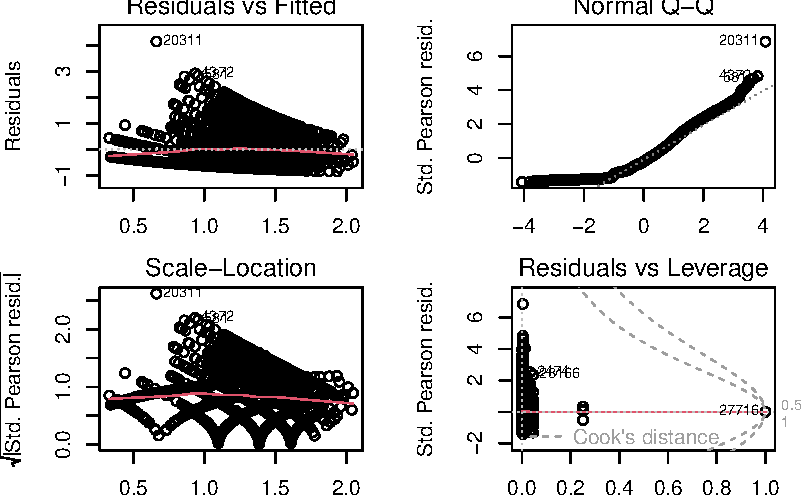
\includegraphics{project_report_files/figure-pdf/unnamed-chunk-45-1.pdf}

}

\end{figure}

\hypertarget{references}{%
\section*{References}\label{references}}
\addcontentsline{toc}{section}{References}

\hypertarget{bibliography-styles}{%
\section{Bibliography styles}\label{bibliography-styles}}

Here are two sample references: \citet{Feynman1963118}
\citet{Dirac1953888}.

By default, natbib will be used with the \texttt{authoryear} style, set
in \texttt{classoption} variable in YAML. You can sets extra options
with \texttt{natbiboptions} variable in YAML header. Example

\begin{verbatim}
natbiboptions: longnamesfirst,angle,semicolon
\end{verbatim}

There are various more specific bibliography styles available at
\url{https://support.stmdocs.in/wiki/index.php?title=Model-wise_bibliographic_style_files}.
To use one of these, add it in the header using, for example,
\texttt{biblio-style:\ model1-num-names}.

\hypertarget{using-csl}{%
\subsection{Using CSL}\label{using-csl}}

If \texttt{cite-method} is set to \texttt{citeproc} in
\texttt{elsevier\_article()}, then pandoc is used for citations instead
of \texttt{natbib}. In this case, the \texttt{csl} option is used to
format the references. By default, this template will provide an
appropriate style, but alternative \texttt{csl} files are available from
\url{https://www.zotero.org/styles?q=elsevier}. These can be downloaded
and stored locally, or the url can be used as in the example header.


  \bibliography{bibliography.bib}


\end{document}
